\documentclass[usenames,dvipsnames,10pt,pdf,utf8,russian,aspectratio=43]{beamer}
\usepackage[english,russian]{babel}
\usepackage{cmap}
\usepackage[T2A]{fontenc}
\usepackage{subfig}
\usepackage{color}
\usepackage{tikz}
%\usepackage{tikz,fullpage}
\DeclareMathOperator*{\argmax}{arg\,max}
\DeclareMathOperator*{\argmin}{arg\,min}

\usetikzlibrary{arrows,automata}
\usetikzlibrary{positioning}

%
% Choose how your presentation looks.
%
% For more themes, color themes and font themes, see:
% http://deic.uab.es/~iblanes/beamer_gallery/index_by_theme.html
%


\mode<presentation>
{


  \usetheme{Boadilla}      % or try Darmstadt, Madrid, Warsaw, ...
  \usecolortheme{seagull} % or try albatross, beaver, crane, ..

 \usefonttheme{structurebold}  % or try serif, structurebold, ...
  \setbeamertemplate{navigation symbols}{}
  \setbeamertemplate{caption}[numbered]
} 


\captionsetup[subfloat]{labelformat=empty}
\title[Выбор структуры]{Выбор структуры модели глубокого обучения}
\author{Бахтеев Олег}
\institute{МФТИ}
\date{06.02.2019}

\begin{document}

\begin{frame}
  \titlepage
\end{frame}


\section{Сложность модели}
\begin{frame}{Сложность модели: зачем?}
\begin{figure}
  \centering
  \subfloat[Устойчивость моделей при возмущении выборки]{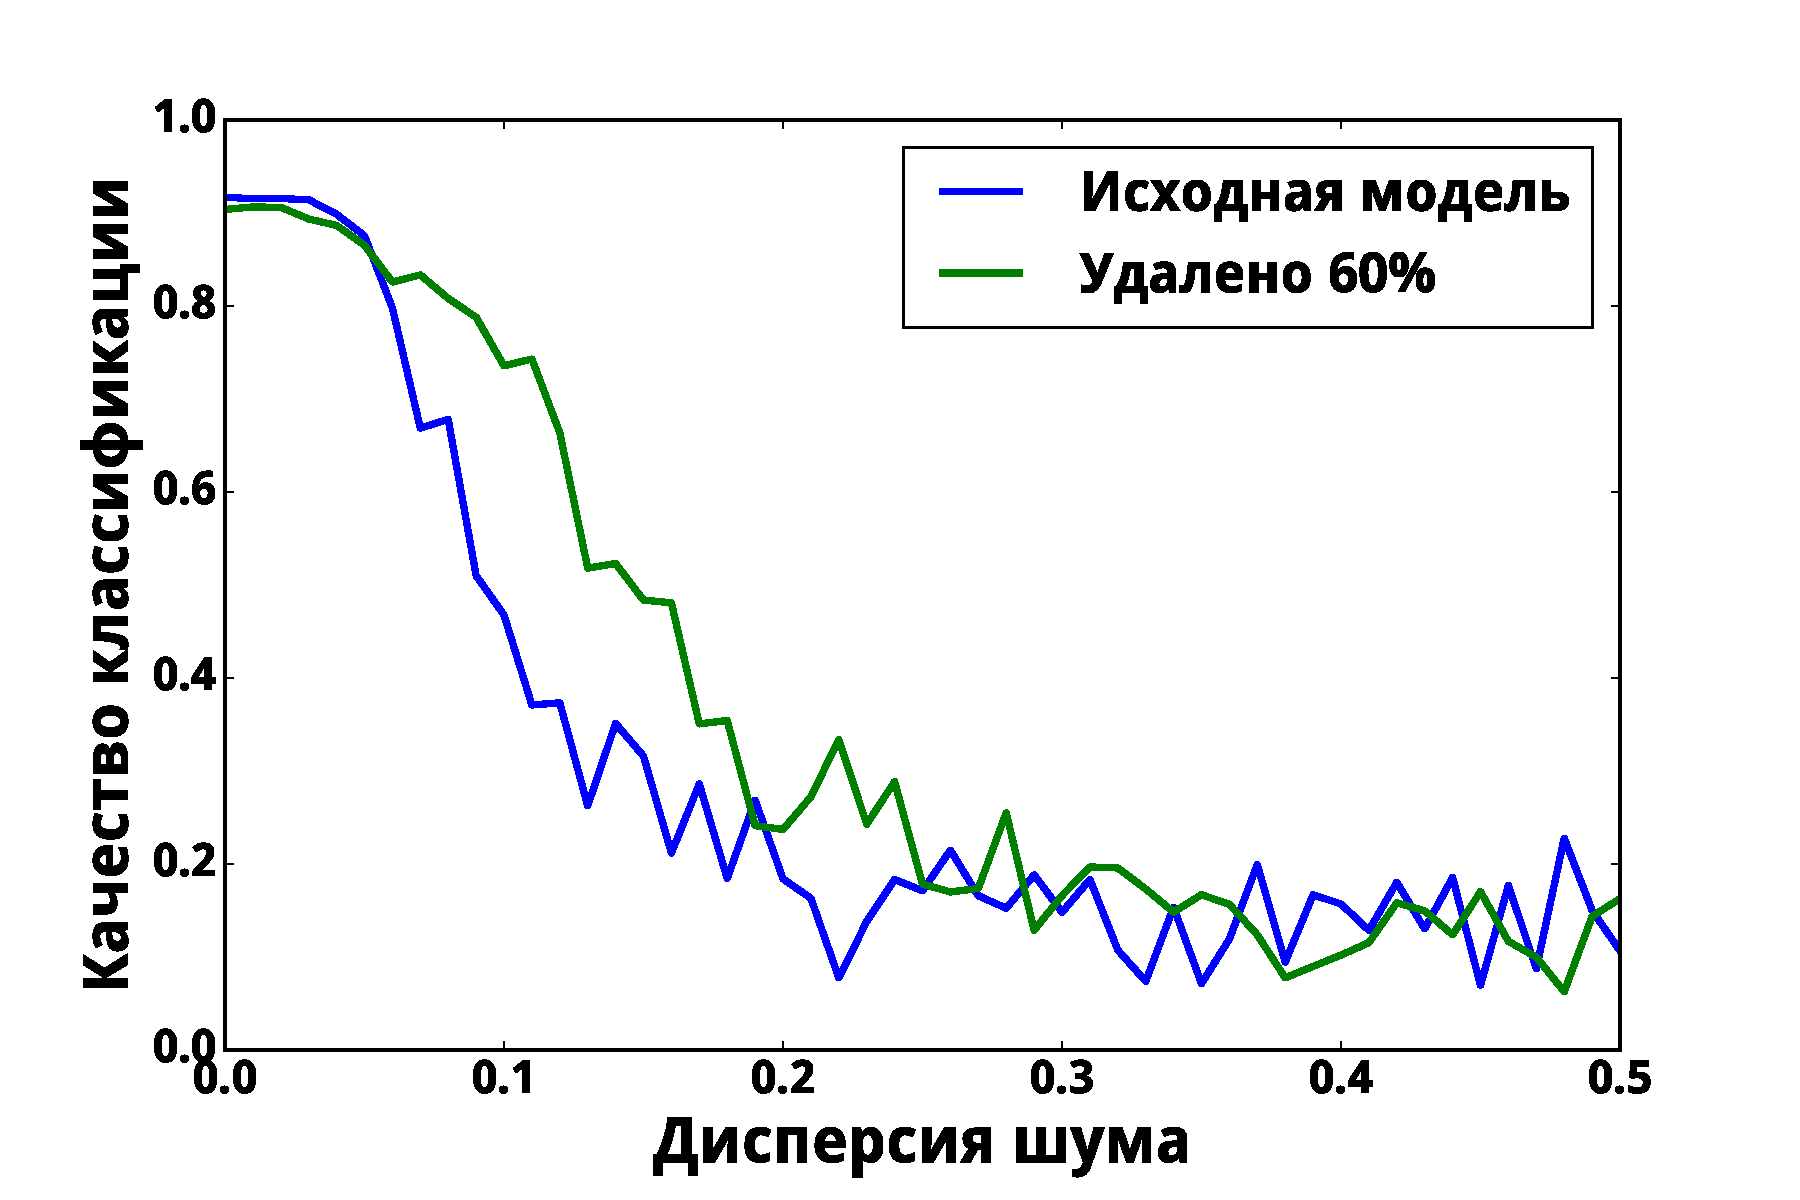
\includegraphics[width=0.4\textwidth]{noise.pdf}} 
 \subfloat[Качество классификации при удалении параметров]{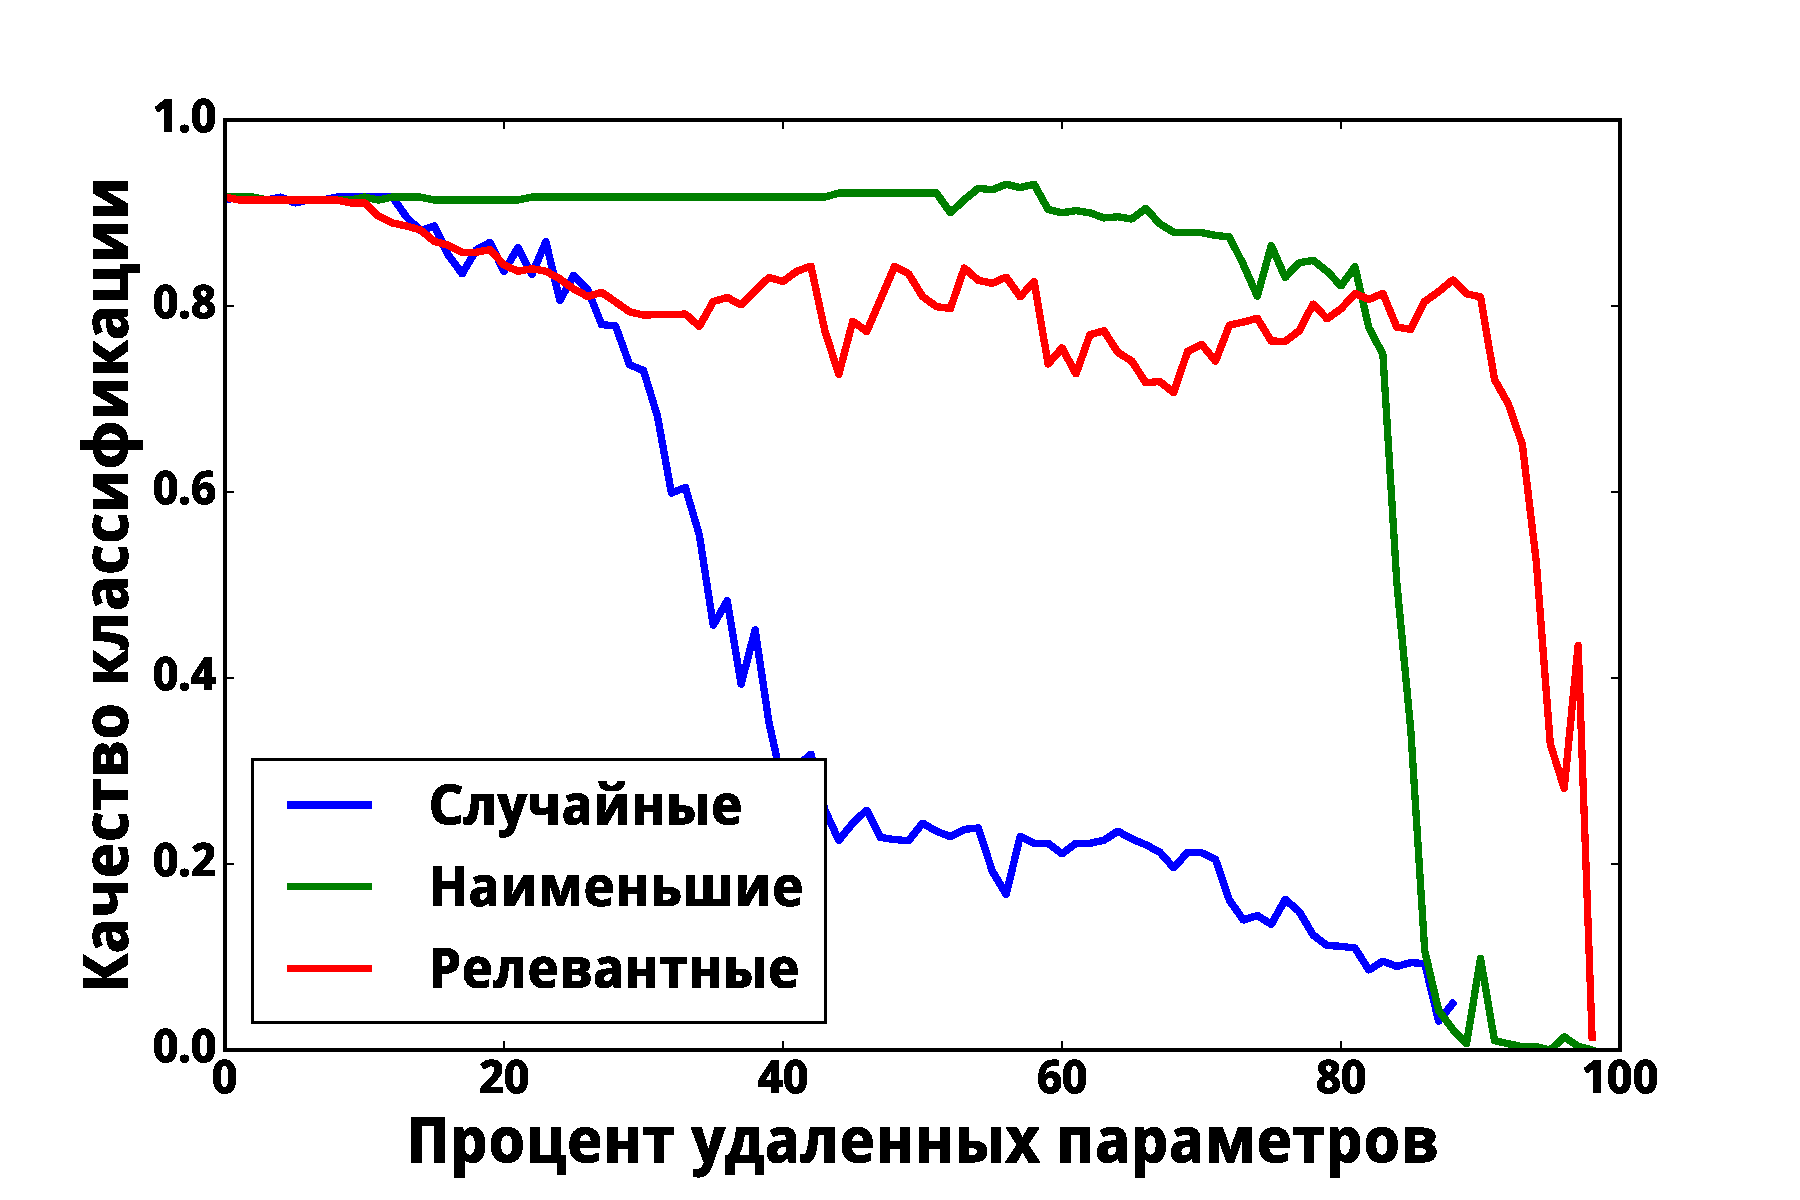
\includegraphics[width=0.4\textwidth]{pruning.pdf}}
\label{fig:1}\qquad

\end{figure}


\end{frame}

\begin{frame}{Сложность модели: зачем?}

\begin{figure}
  \centering
 {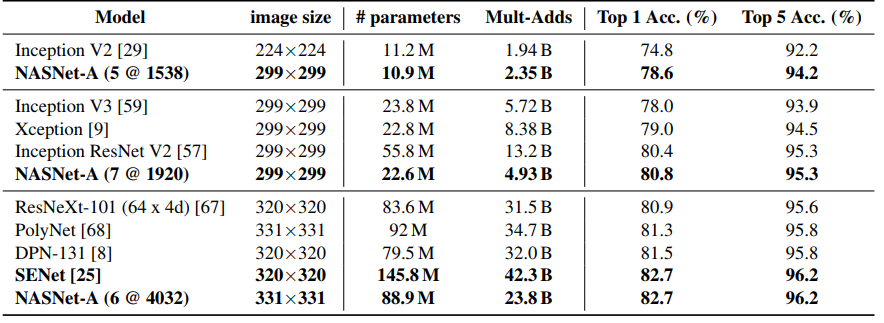
\includegraphics[width=\textwidth]{zoph.png}}
\label{fig:1}\qquad
\caption*{Zoph et. al, 2017.  Сложность моделей отличается почти в два раза при одинаковом качестве.}
\end{figure}
\end{frame}

\begin{frame}{Глубокого обучение}
\begin{block}{Определение}
\textit{Моделью} $\mathbf{f}(\mathbf{w}, \mathbf{x})$ назовем дифференцируемую по параметрам $\mathbf{w}$ функцию из множества признаковых описаний объекта во множество меток:
\[
    \mathbf{f}: \mathbb{X} \times \mathbb{W} \to \mathbb{Y},
\] 
где $\mathbb{W}$ --- пространство параметров функции $\mathbf{f}$.
\end{block}
~\\~\\
\textbf{Особенность задачи}  выбора модели \textit{глубокого обучения} --- значительное число параметро в моделях приводит к неприменимости классических методов оптимизации и выбора модели. \\~\\

\textbf{Сложность модели:}
\begin{enumerate}
\item количество параметров;
\item количество суперпозиций внутри модели.
\end{enumerate}
\end{frame}


\begin{frame}{Принцип минимальной длины описания}
\[
\text{MDL}(\mathbf{f}, \mathfrak{D}) = L(\mathbf{f}) + L(\mathfrak{D}|\mathbf{f}),
\]
где $\mathbf{f}$ --- модель, $\mathfrak{D}$ --- выборка, $L$ --- длина описания в битах.
\\
\[
\text{MDL}(\mathbf{f}, \mathfrak{D}) \sim L(\mathbf{f}) + L(\mathbf{w}^*| \mathbf{f}) + L(\mathfrak{D}|\mathbf{w}^*, \mathbf{f}),
\]
$\mathbf{w}^*$ --- оптимальные параметры модели.\\

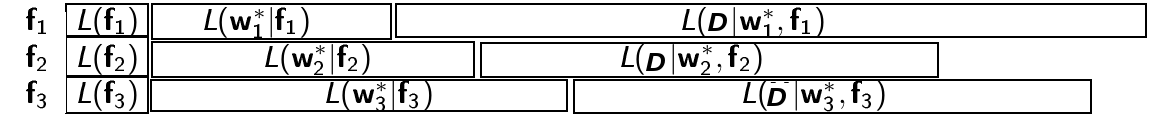
\includegraphics[width=\textwidth]{./mdl.png}

\end{frame}

\begin{frame}{MDL и Колмогоровская сложность}
\textbf{Колмогоровская сложность} --- длина минимального кода для выборки на предварительно заданном языке.

\textbf{Теорема инвариантности}\\
Для двух сводимых по Тьюрингу языков колмогоровская сложность  отличается не более чем на константу, не зависяющую от мощности выборки.\\

\textbf{Отличия от MDL}:
\begin{itemize}
\item Колмогоровская сложность невычислима.
\item Длина кода может зависеть от выбранного языка. Для небольших выборок теорема инвариантности не дает адекватных результатов.
\end{itemize}
\end{frame}



\begin{frame}{Байесовый подход к сложности}
Правдоподобие модели (``Evidence''):
\[
	p(\mathfrak{D}|\mathbf{h}) = \int_\mathbf{w} p(\mathfrak{D}|\mathbf{w})p(\mathbf{w}|\mathbf{h}) d\mathbf{w}.
\]


\begin{figure}
  \centering
  \subfloat[Схема выбора модели по правдоподобию]{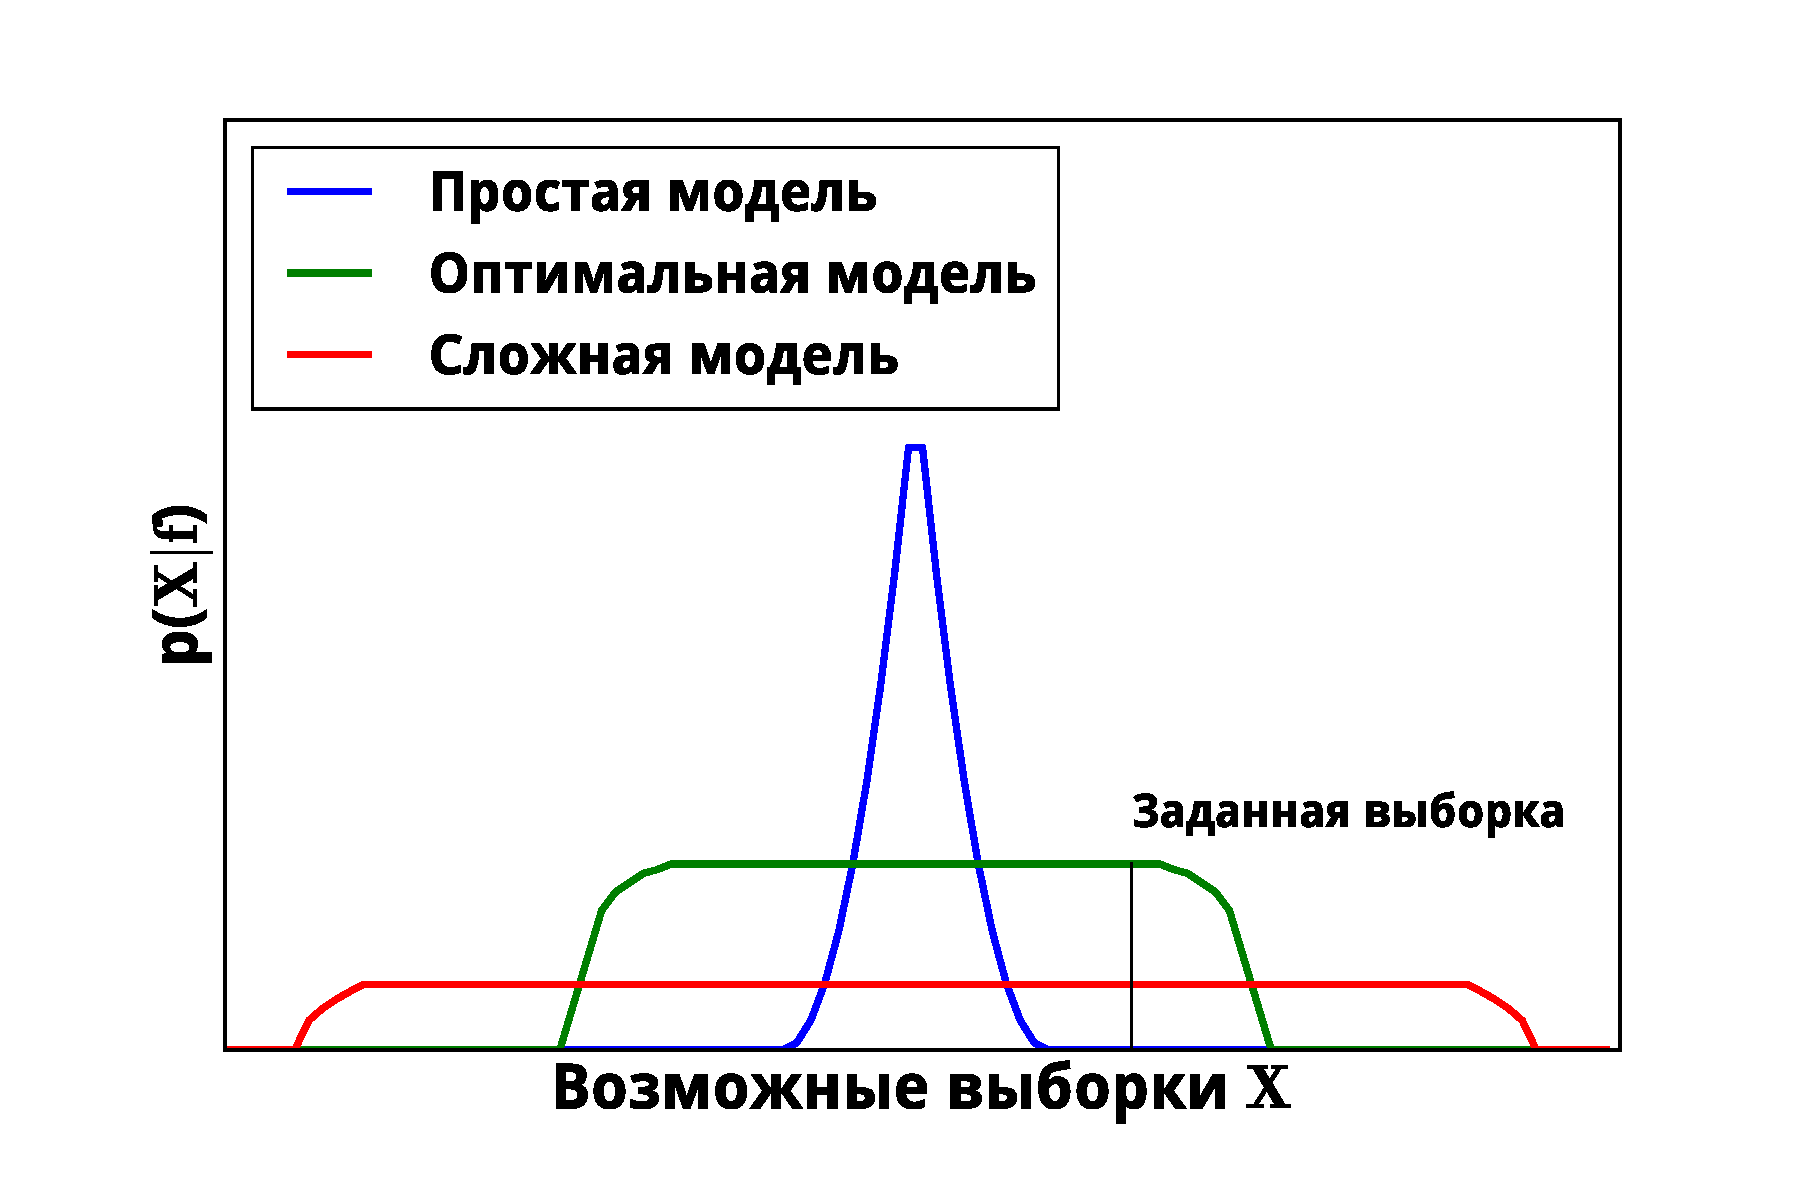
\includegraphics[width=0.4\textwidth]{evidence.pdf}} 
 \subfloat[Пример: полиномы]{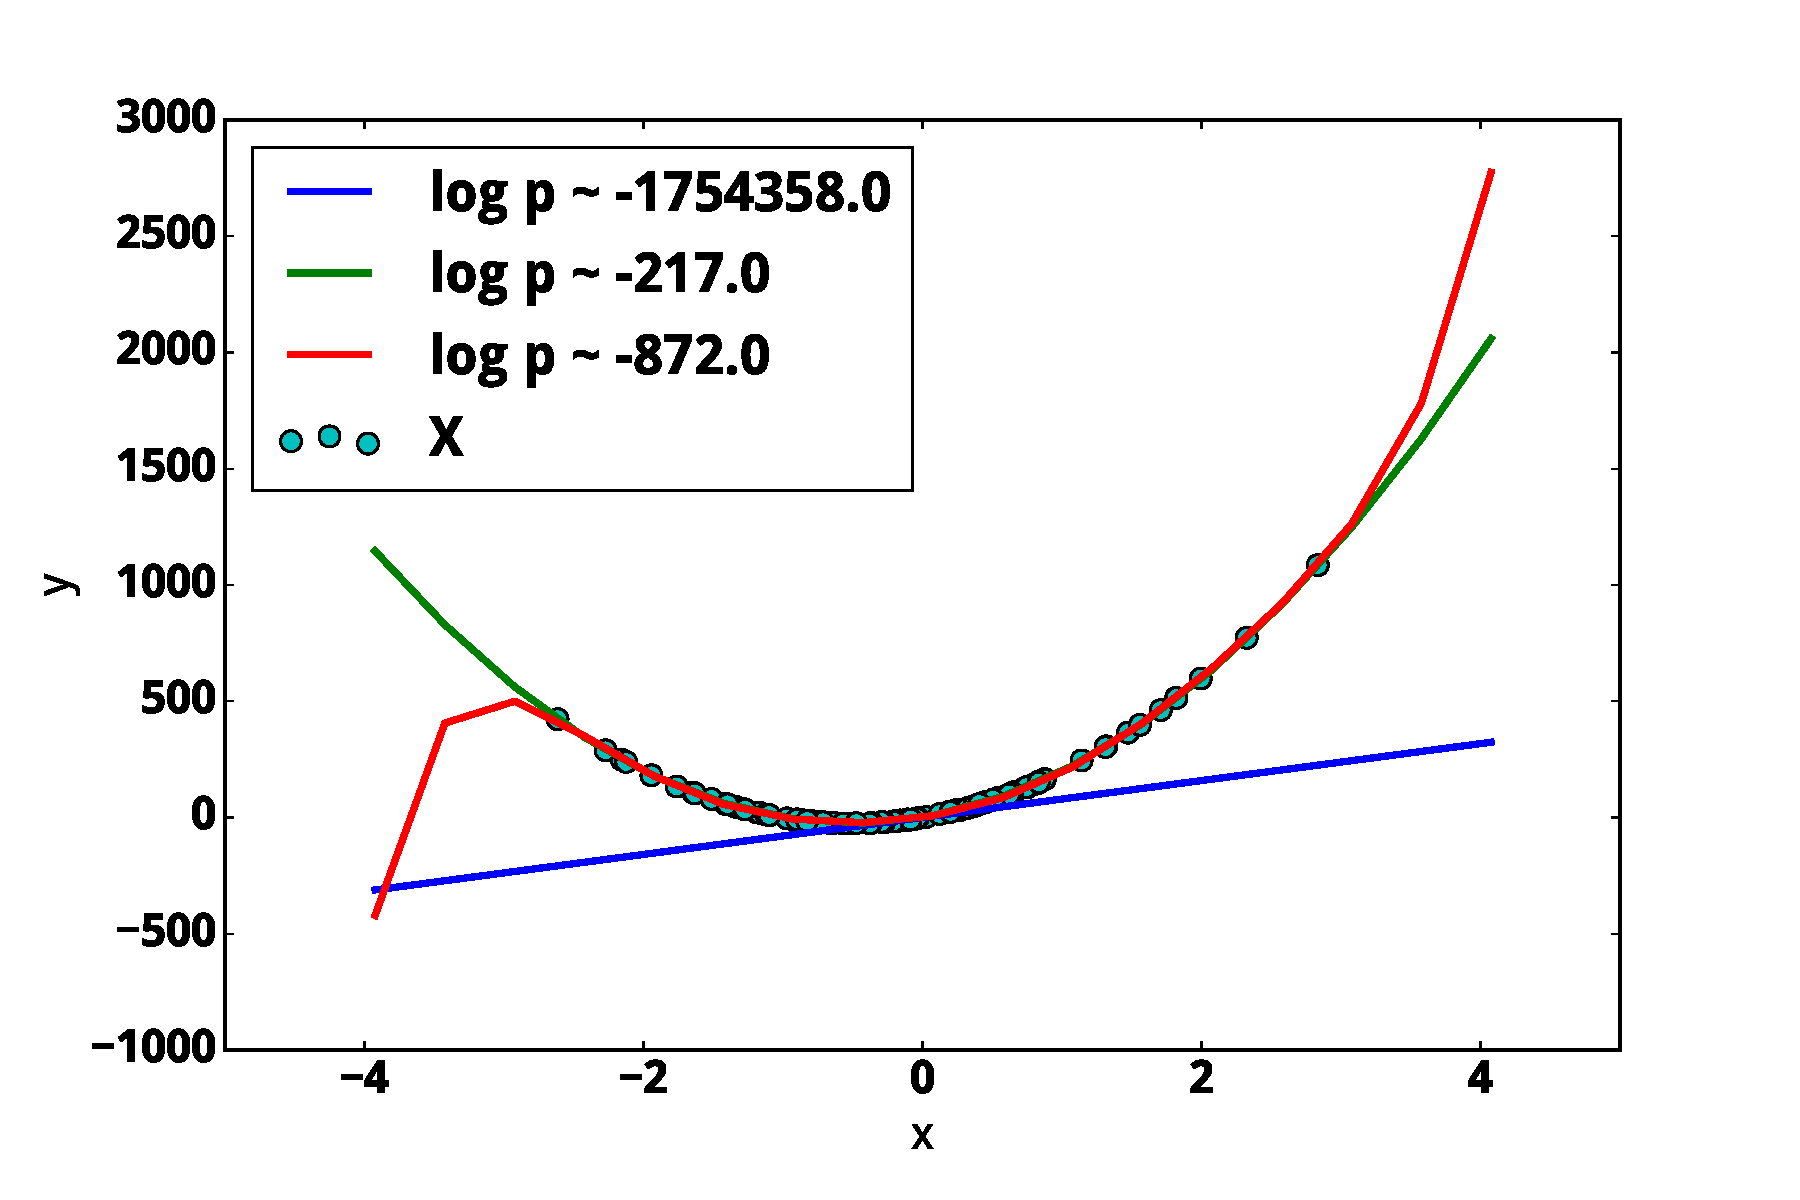
\includegraphics[width=0.4\textwidth]{example.pdf}}
\label{fig:1}\qquad

\end{figure}


\end{frame}

\begin{frame}{Evidence vs MDL}
\small
\begin{tabular}{ c | c  }
  \hline			
 \bf Evidence & \bf MDL \\
  \hline  
Использует априорные знания &  Независима от априорных знаний \\
  \hline  
Основывается на гипотезе о порождении\\ выборки & Минимизирует длину описания выборки\\ вне зависимости от их природы \\
  \hline  

\end{tabular}


\begin{figure}
  \centering
 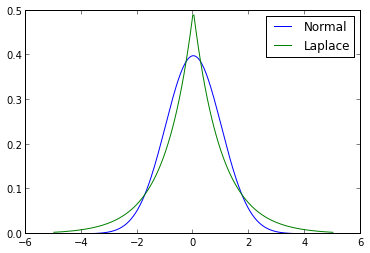
\includegraphics[width=0.4\textwidth]{laplace.png}
\label{fig:1}\qquad

\end{figure}


\end{frame}



\begin{frame}{Оптимальность модели}
\begin{block}{Определение}
Пусть задано множество моделей $M$.  \\
Пусть для каждой модели $\mathbf{f}$ задано априорное распределение параметров: $p(\mathbf{w}|\mathbf{h})$, где $\mathbf{h}$ --- параметры априорного распределения.\\
Модель $\mathbf{f}$ назовем оптимальной среди моделей ${M}$, если достигается максимум интеграла:
\[
	p(\mathfrak{D}|\mathbf{h}) = \int_\mathbf{w} p(\mathfrak{D}|\mathbf{w})p(\mathbf{w}|\mathbf{h}) d\mathbf{w}.
\]
\end{block}
\end{frame}




\section{Вариационная нижняя оценка}
\begin{frame}{Вариационная оценка, ELBO}
%http://www.orchid.ac.uk/eprints/40/1/fox_vbtut.pdf
\textbf{Вариационная оценка Evidence}, Evidence lower bound --- метод нахождения приближенного значения аналитически невычислимого распределения $p(\mathbf{w}|\mathfrak{D}, \mathbf{h})$ распределением $q(\mathbf{w}) \in \mathbf{Q}$. Получение вариационной нижней оценки обычно сводится к задаче минимизации
$$\text{KL}(q(\mathbf{w})||p(\mathbf{w}| \mathfrak{D}))=
-\int_{\mathbf{w}} q(\mathbf{w}) \text{log}~\frac{p(\mathbf{w}| \mathfrak{D})} {q(\mathbf{w})}d\mathbf{w}.
$$

\begin{figure}
  \centering
  \subfloat[Аппроксимация неизвестного распределения нормальным]{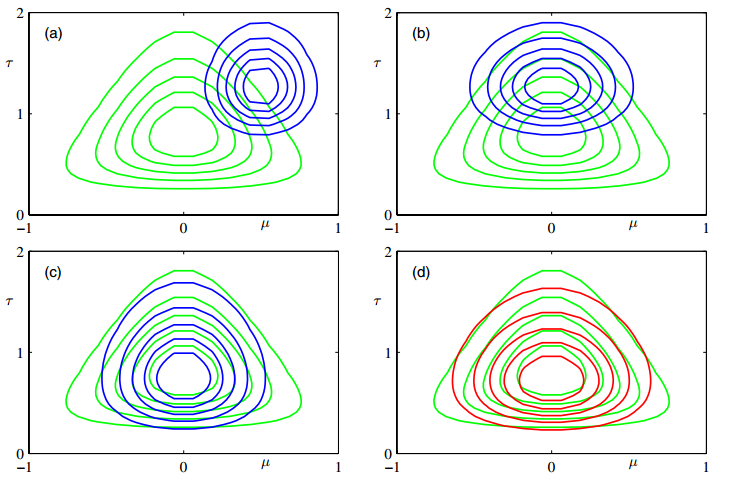
\includegraphics[width=0.33\textwidth]{omnomnom.png}} 
 \subfloat[Аппроксимация Лапласа (красная линия) и вариационная оценка (зеленая линия)]{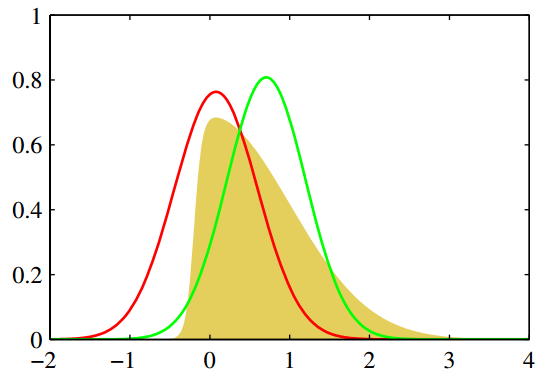
\includegraphics[width=0.33\textwidth]{laplace_vs_var.png}}
\label{fig:1}\qquad

\end{figure}

\end{frame}

\begin{frame}{Получение вариацонной нижней оценки}
$$
\text{log}~p(\mathfrak{D}| \mathbf{h})  = \int_{\mathbf{w}} q(\mathbf{w})\text{log}~\frac{p(\mathfrak{D},\mathbf{w}|\mathbf{h})}{q(\mathbf{w})}d\mathbf{w} + \text{D}_\text{KL}  (q(\mathbf{w})||p(\mathbf{w}| \mathfrak{D}, \mathbf{h})) \geq	
$$
$$
\geq \int_{\mathbf{w}} q(\mathbf{w})\text{log}~\frac{p(\mathfrak{D},\mathbf{w}|\mathbf{h})}{q(\mathbf{w})}d\mathbf{w} =
$$

$$
= -\text{D}_\text{KL} (q(\mathbf{w})||p(\mathbf{w}|\mathbf{h})) + \int_{\mathbf{w}} q(\mathbf{w})\text{log}~{p(\mathfrak{D}|\mathbf{w},\mathbf{h})} d \mathbf{w},
$$
где $$\text{D}_\text{KL}(q(\mathbf{w})||p(\mathbf{w} |\mathbf{h})) = -\int_{\mathbf{w}} q(\mathbf{w})\text{log}~\frac{p(\mathbf{w} | \mathbf{h})}{q(\mathbf{w})}d\mathbf{w}.$$
\begin{block}{Определение} Модель $\mathbf{f}$ назовем субоптимальной на множестве моделей $M$, если модель доставляет максимум нижней вариационной оценке:
\[
\label{eq:elbo2}
	\mathbf{f} = \argmax_{\hat{\mathbf{f}} \in M}\max_{q \in {Q}}\int_{\mathbf{w}} q(\mathbf{w})\textnormal{log}~\frac{p(\mathbf{y},\mathbf{w}|\mathfrak{D},\hat{\mathbf{f})}}{q(\mathbf{w})}d\mathbf{w}.
\]
\end{block}


\end{frame}

\begin{frame}{$D_\text{KL}$}
Максимизация вариационной нижней оценки $$\int_{\mathbf{w}} q(\mathbf{w})\text{log}~\frac{p(\mathfrak{D},\mathbf{w}|\mathbf{h})}{q(\mathbf{w})}d\mathbf{w}$$   эквивалентна минимизации дивергенции между распределением распределением $q(\mathbf{w}) \in Q$ и апостериорным распределением параметров $p(\mathbf{w}|\mathfrak{D}, \mathbf{h})$:
\[
q = \text{argmax}_{q \in Q}\int_{\mathbf{w}} q(\mathbf{w})\text{log}~\frac{p(\mathfrak{D},\mathbf{w}|\mathbf{h})}{q(\mathbf{w})}d\mathbf{w} \Leftrightarrow 	
q = \text{argmin}_{q \in Q} \text{D}_\text{KL}  (q(\mathbf{w})||p(\mathbf{w}| \mathfrak{D}, \mathbf{h})),
\]
т.к.
$$\text{log}~p(\mathfrak{D}| \mathbf{h})  = \int_{\mathbf{w}} q(\mathbf{w})\text{log}~\frac{p(\mathfrak{D},\mathbf{w}|\mathbf{h})}{q(\mathbf{w})}d\mathbf{w} + \text{D}_\text{KL}  (q(\mathbf{w})||p(\mathbf{w}| \mathfrak{D}, \mathbf{h})) = \text{const}.$$



\end{frame}



\begin{frame}{Использование вариационной нижней оценки}
\textbf{Для чего используют вариационный вывод?}
\begin{itemize}
\item получение оценок Evidence;
\item получение оценок распределений моделей со скрытыми переменными (тематическое моделирование, снижение размерности).
\end{itemize}

\textbf{Зачем используют вариационный вывод?}
\begin{itemize}
\item сводит задачу нахождения апостериорной вероятности к методам оптимизации;
\item проще масштабируется, чем аппроксимация Лапласа;
\item проще в использовании, чем сэмплирующие методы.
\end{itemize}
\textbf{Вариационный вывод может давать сильно заниженную оценку.}
\end{frame}


\section{Получение оценок для разделяющих моделей}
\begin{frame}{ELBO: нормальное распределение}
Пусть $q \sim \mathcal{N}(\boldsymbol{\mu}_q, \mathbf{A}_q).$\\
Тогда вариационная оценка имеет вид:
$$
\int_{\mathbf{w}} q(\mathbf{w})\text{log}~{p(\mathbf{Y}|\mathbf{X},\mathbf{w},\mathbf{h})} d \mathbf{w} - D_\text{KL}\bigl(q (\mathbf{w} )|| p (\mathbf{w}|\mathbf{h})\bigr) \simeq
$$
$$
\sum_{i=1}^m \text{log}~p(\mathbf{y}_i|\mathbf{x}_i, \hat{\mathbf{w}}) - D_\text{KL}\bigl(q (\mathbf{w} )|| p (\mathbf{w}|\mathbf{h})\bigr) \to \max_{\mathbf{A}_q, \boldsymbol{\mu}_q}, \quad \hat{\mathbf{w}} \sim q.
$$
В случае, если априорное распределение параметров $p(\mathbf{w}|\mathbf{h})$ является нормальным: 
$$
p(\mathbf{w}|\mathbf{h}) \sim \mathcal{N}(\boldsymbol{\mu}, \mathbf{A}),
$$
дивергенция $D_\text{KL}\bigl(q (\mathbf{w} )|| p (\mathbf{w}|\mathbf{h})$ вычисляется аналитически:
$$
D_\text{KL}\bigl(q (\mathbf{w}) || p (\mathbf{w}|\mathbf{h})\bigr) = \frac{1}{2} \bigl( \text{tr} (\mathbf{A}^{-1}\mathbf{A}_q) + (\boldsymbol{\mu} - \boldsymbol{\mu}_q)^\text{T}\mathbf{A}^{-1}(\boldsymbol{\mu} - \boldsymbol{\mu}_q) - n +\text{ln}~|\mathbf{A}| - \text{ln}~|\mathbf{A}_q| \bigr).
$$
\end{frame}



\begin{frame}{ELBO: нормальное распределение}
\begin{columns}[T] 
\begin{column}{.48\textwidth}
\textbf{``Обычная'' функция потерь:}\\
$$
L = \textcolor{red}{\sum_{\mathbf{x}, \mathbf{y} \in \mathfrak{D}} - \text{log}p(\mathbf{y}|\mathbf{x}, \mathbf{w})} + \textcolor{blue}{\lambda||\mathbf{w}||_2^2}.
$$\\~\\

% если n - константна.
\textbf{Вариационный вывод при $(p(\mathbf{w}|\mathbf{h}) \sim \mathcal{N}(\mathbf{0}, \mathbf{1}))$:}\\
$$
L =   \textcolor{red}{\sum_{\mathbf{x}, \mathbf{y}} \text{log}~p(\mathbf{y}|\mathbf{x}, \hat{\mathbf{w}})} +
$$
$$ + \textcolor{blue}{\frac{1}{2} \bigl( \text{tr} (\mathbf{A}_q) + \boldsymbol{\mu}_q^\text{T}\mathbf{A}^{-1}\boldsymbol{\mu}_q  - \text{ln}~|\mathbf{A}_q| \bigr)}.
$$\\~\\

\end{column}%
\hfill%
\begin{column}{.48\textwidth}

\begin{center}
\begin{figure}
\caption*{Пример грубой аппроксимации нормальным диагональным распределением $q$}
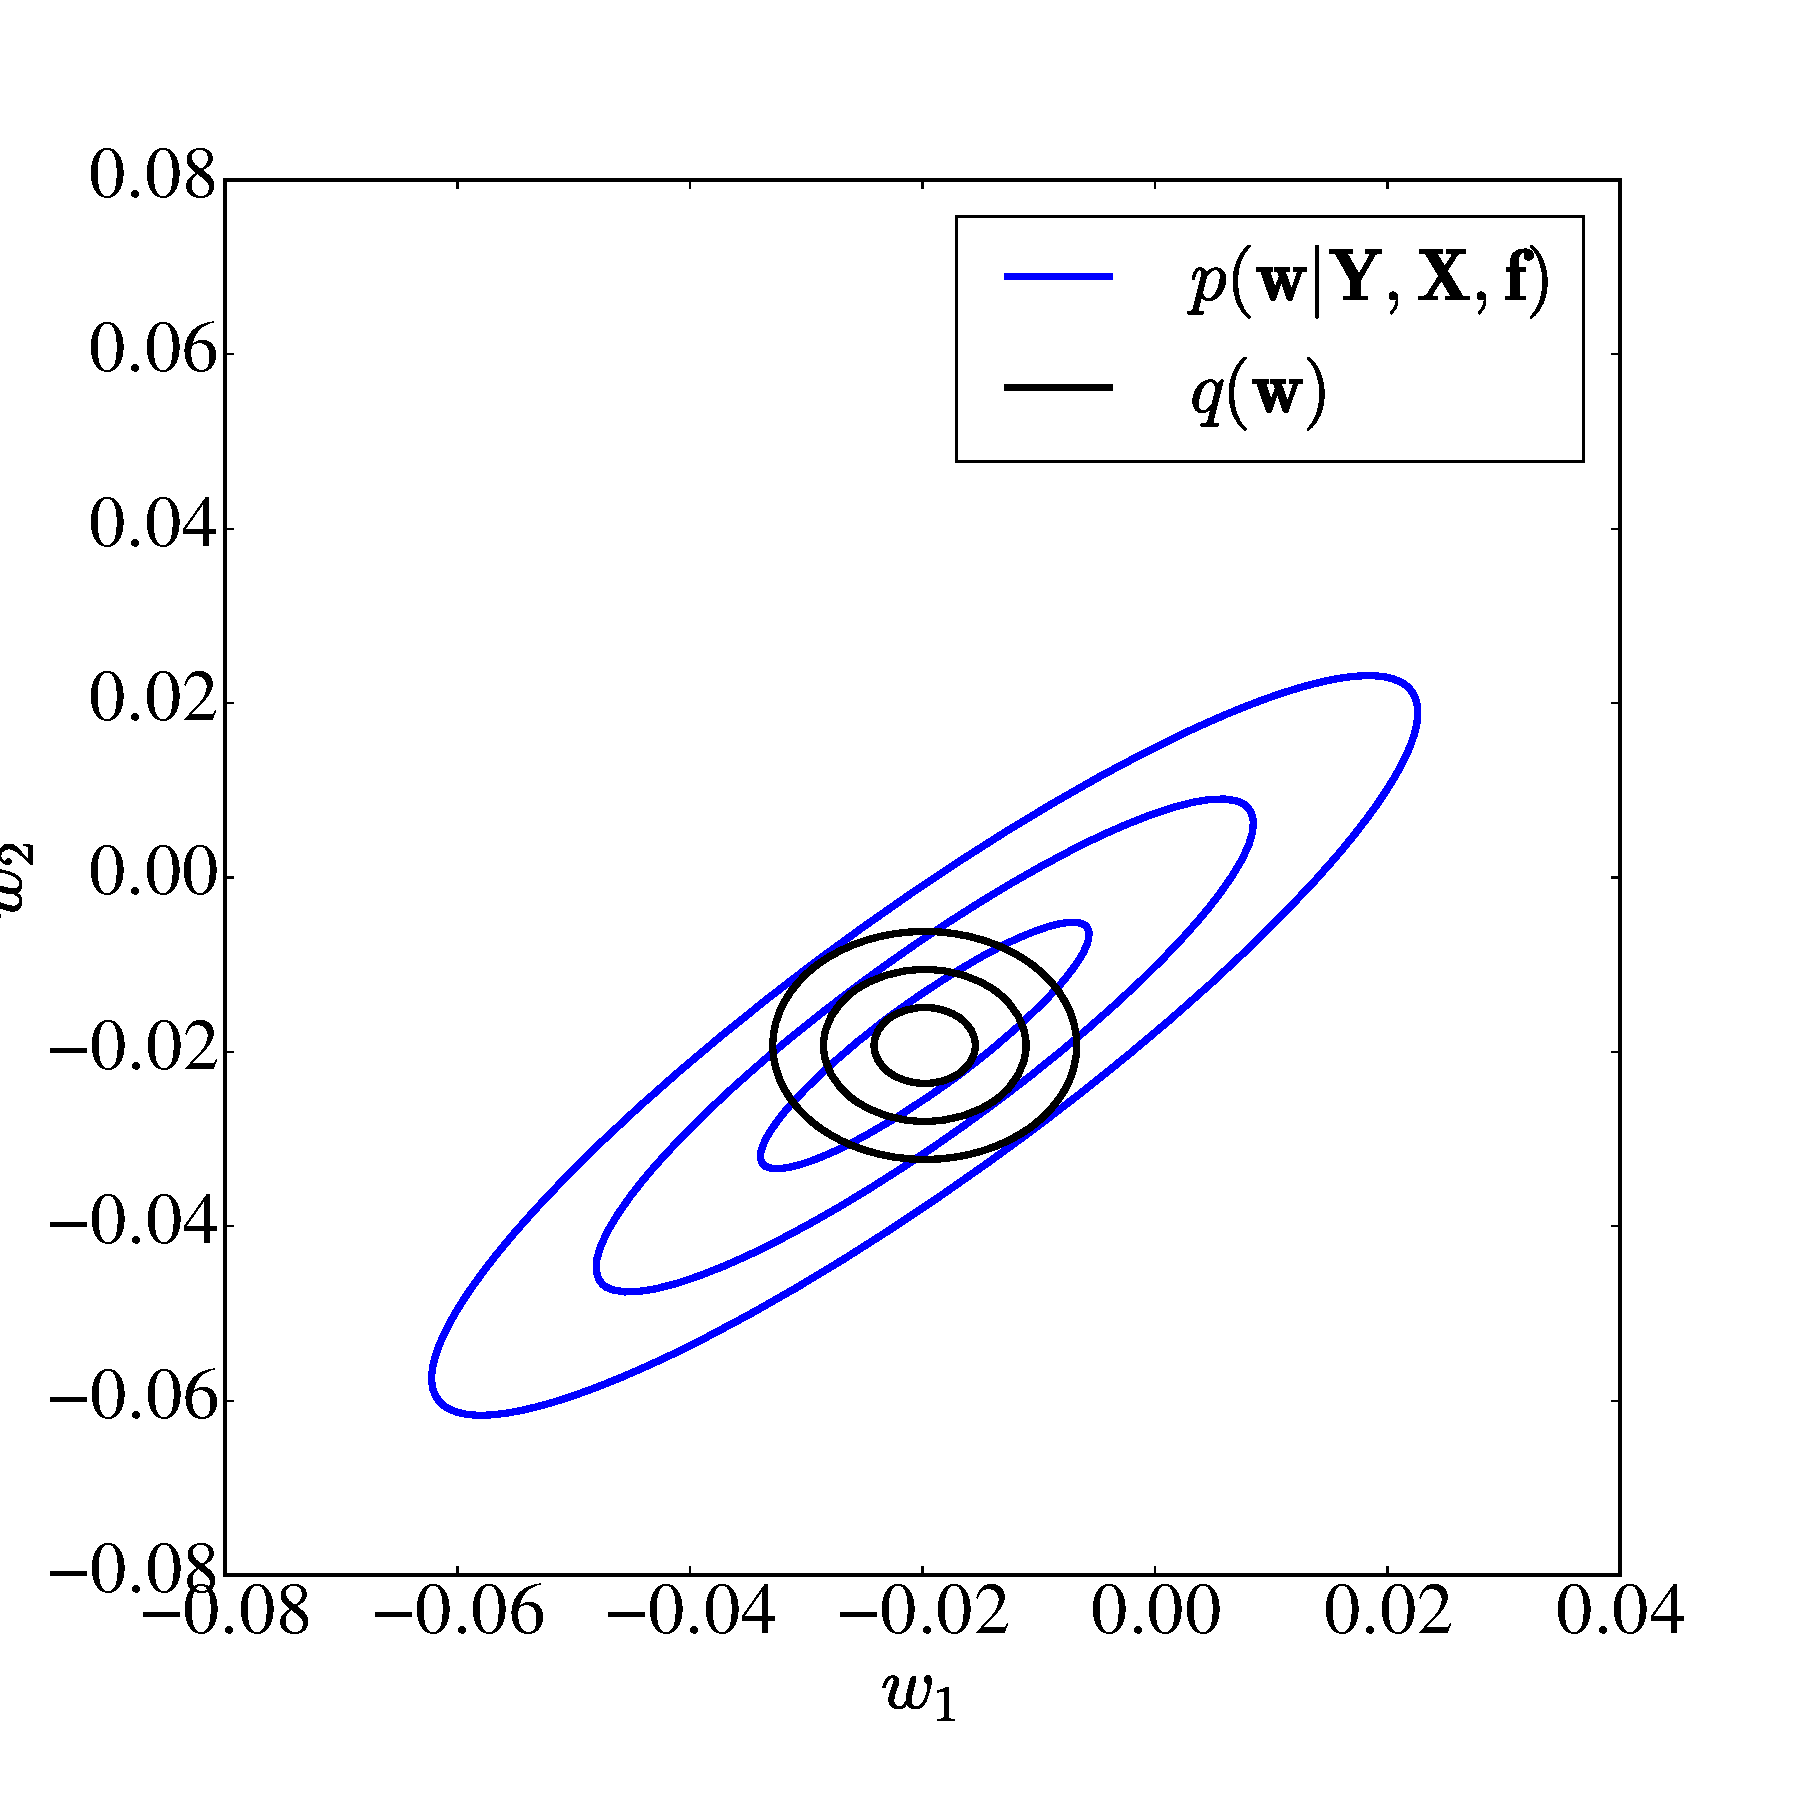
\includegraphics[width=0.8\textwidth]{mf.pdf}
\end{figure}
\end{center}

\end{column}%
\end{columns}

\end{frame}








\begin{frame}{Оператор оптимизации, Maclaurin et. al, 2015}
\begin{block}{Определение}
Назовем оператором оптимизации алгоритм $T$ выбора вектора параметров $\mathbf{w}'$  по параметрам предыдущего шага $\mathbf{w}$:
\[
	\mathbf{w}' = T(\mathbf{w}).
\]
\end{block}

\begin{block}{Определение}
Пусть $L$ --- дифференцируемая функция потерь. \\
Оператором градиентного спуска назовем следующий оператор:
\[
    T(\mathbf{w}) = \mathbf{w} - \beta \nabla L(\mathbf{w}, \mathbf{y}, \mathfrak{D}).
\]
\end{block}


\end{frame}

\begin{frame}{Градиентный спуск для оценки правдоподобия}
Рассмотрим максимизацию совместного распределения параметров:
\[
    L =  -\text{log}~p(\mathfrak{D},\mathbf{w}|\mathbf{h}) = -\sum_{\mathfrak{D} \in \mathfrak{D}} \text{log}~p(\mathfrak{D}|\mathbf{w}, \mathbf{h}) p(\mathbf{w}|\mathbf{h})
\]
Проведем оптимизацию нейросети  из $r$ различных начальных приближений $\mathbf{w}_1, \dots, \mathbf{w}_r$ с использованием градиентного спуска:
\[
\mathbf{w}' = T(\mathbf{w}).
\]

Векторы параметров $\mathbf{w}_1,\dots,\mathbf{w}_r$ соответствуют некоторому скрытому распределению $q(\mathbf{w})$.

\end{frame}



\begin{frame}{Энтропия}
Формулу вариационной оценки можно переписать с использованием энтропии:
$$\text{log}~p(\mathfrak{D}|\mathbf{f}) \geq 
\int_{\mathbf{w}} q(\mathbf{w})\text{log}~\frac{p(\mathfrak{D},\mathbf{w}|\mathbf{h})}{q(\mathbf{w})}d\mathbf{w} = 
$$
$$
\mathsf{E}_{q(\mathbf{w)}}[\text{log~}p (\mathfrak{D}, \mathbf{w}| \mathbf{h})] + \mathsf{S}({q(\mathbf{w)}}),
$$
где $\mathsf{S}({q(\mathbf{w)}})$ --- энтропия:
$$
\mathsf{S}({q(\mathbf{w)}}) = - \int_{\mathbf{w}} q(\mathbf{w})\text{log}~q(\mathbf{w})d\mathbf{w}.  	
$$
\end{frame}


\begin{frame}{Градиентный спуск для оценки правдоподобия}
При достаточно малой длине шага оптимизации $\beta$ разность энтропии на различных шагах оптимизации вычисляется как:
\[
\mathsf{S}(q'(\mathbf{w})) -  \mathsf{S}(q(\mathbf{w}))  \simeq  \frac{1}{r}\sum_{g=1}^r \bigl(-\beta \text{Tr}[\mathbf{H}(\mathbf{w}'^g)] - \beta^2 \text{Tr}[\mathbf{H}(\mathbf{w}'^g)\mathbf{H}(\mathbf{w}'^g)]  \bigr).
\]

Итоговая оценка на шаге оптимизации $\tau$:
$$
\text{log}~\hat{p}(\mathbf{Y}|\mathfrak{D}, \mathbf{h}) \sim \frac{1}{r} \sum_{g = 1}^r L(\mathbf{w}^g_\tau, \mathfrak{D}, \mathbf{Y})  + \mathsf{S}(q^0(\mathbf{w}))+$$ $$ + \frac{1}{r}\sum_{b=1}^\tau\sum_{g=1}^r \bigl(-\beta \text{Tr}[\mathbf{H}(\mathbf{w}_b^g)] - \beta^2 \text{Tr}[\mathbf{H}(\mathbf{w}_b^g)\mathbf{H}(\mathbf{w}_b^g)]  \bigr),
$$
$\mathbf{w}_b^g$ --- вектор параметров старта $g$ на шаге $b$, $\mathsf{S}(q^0(\mathbf{w}))$ --- начальная энтропия.
\end{frame}
\begin{frame}{Переобучение,  Maclaurin et. al, 2015}
Градиентный спуск не минимизирует дивергенцию $\text{KL}(q(\mathbf{w})||p(\mathbf{w}| \mathfrak{D}, \mathbf{h}))$. При приближении к моде распределения снижается оценка Evidence, что интерпретируется как переоубчение модели.

\begin{figure}
  \centering
  \subfloat[Схождение распределения к моде]{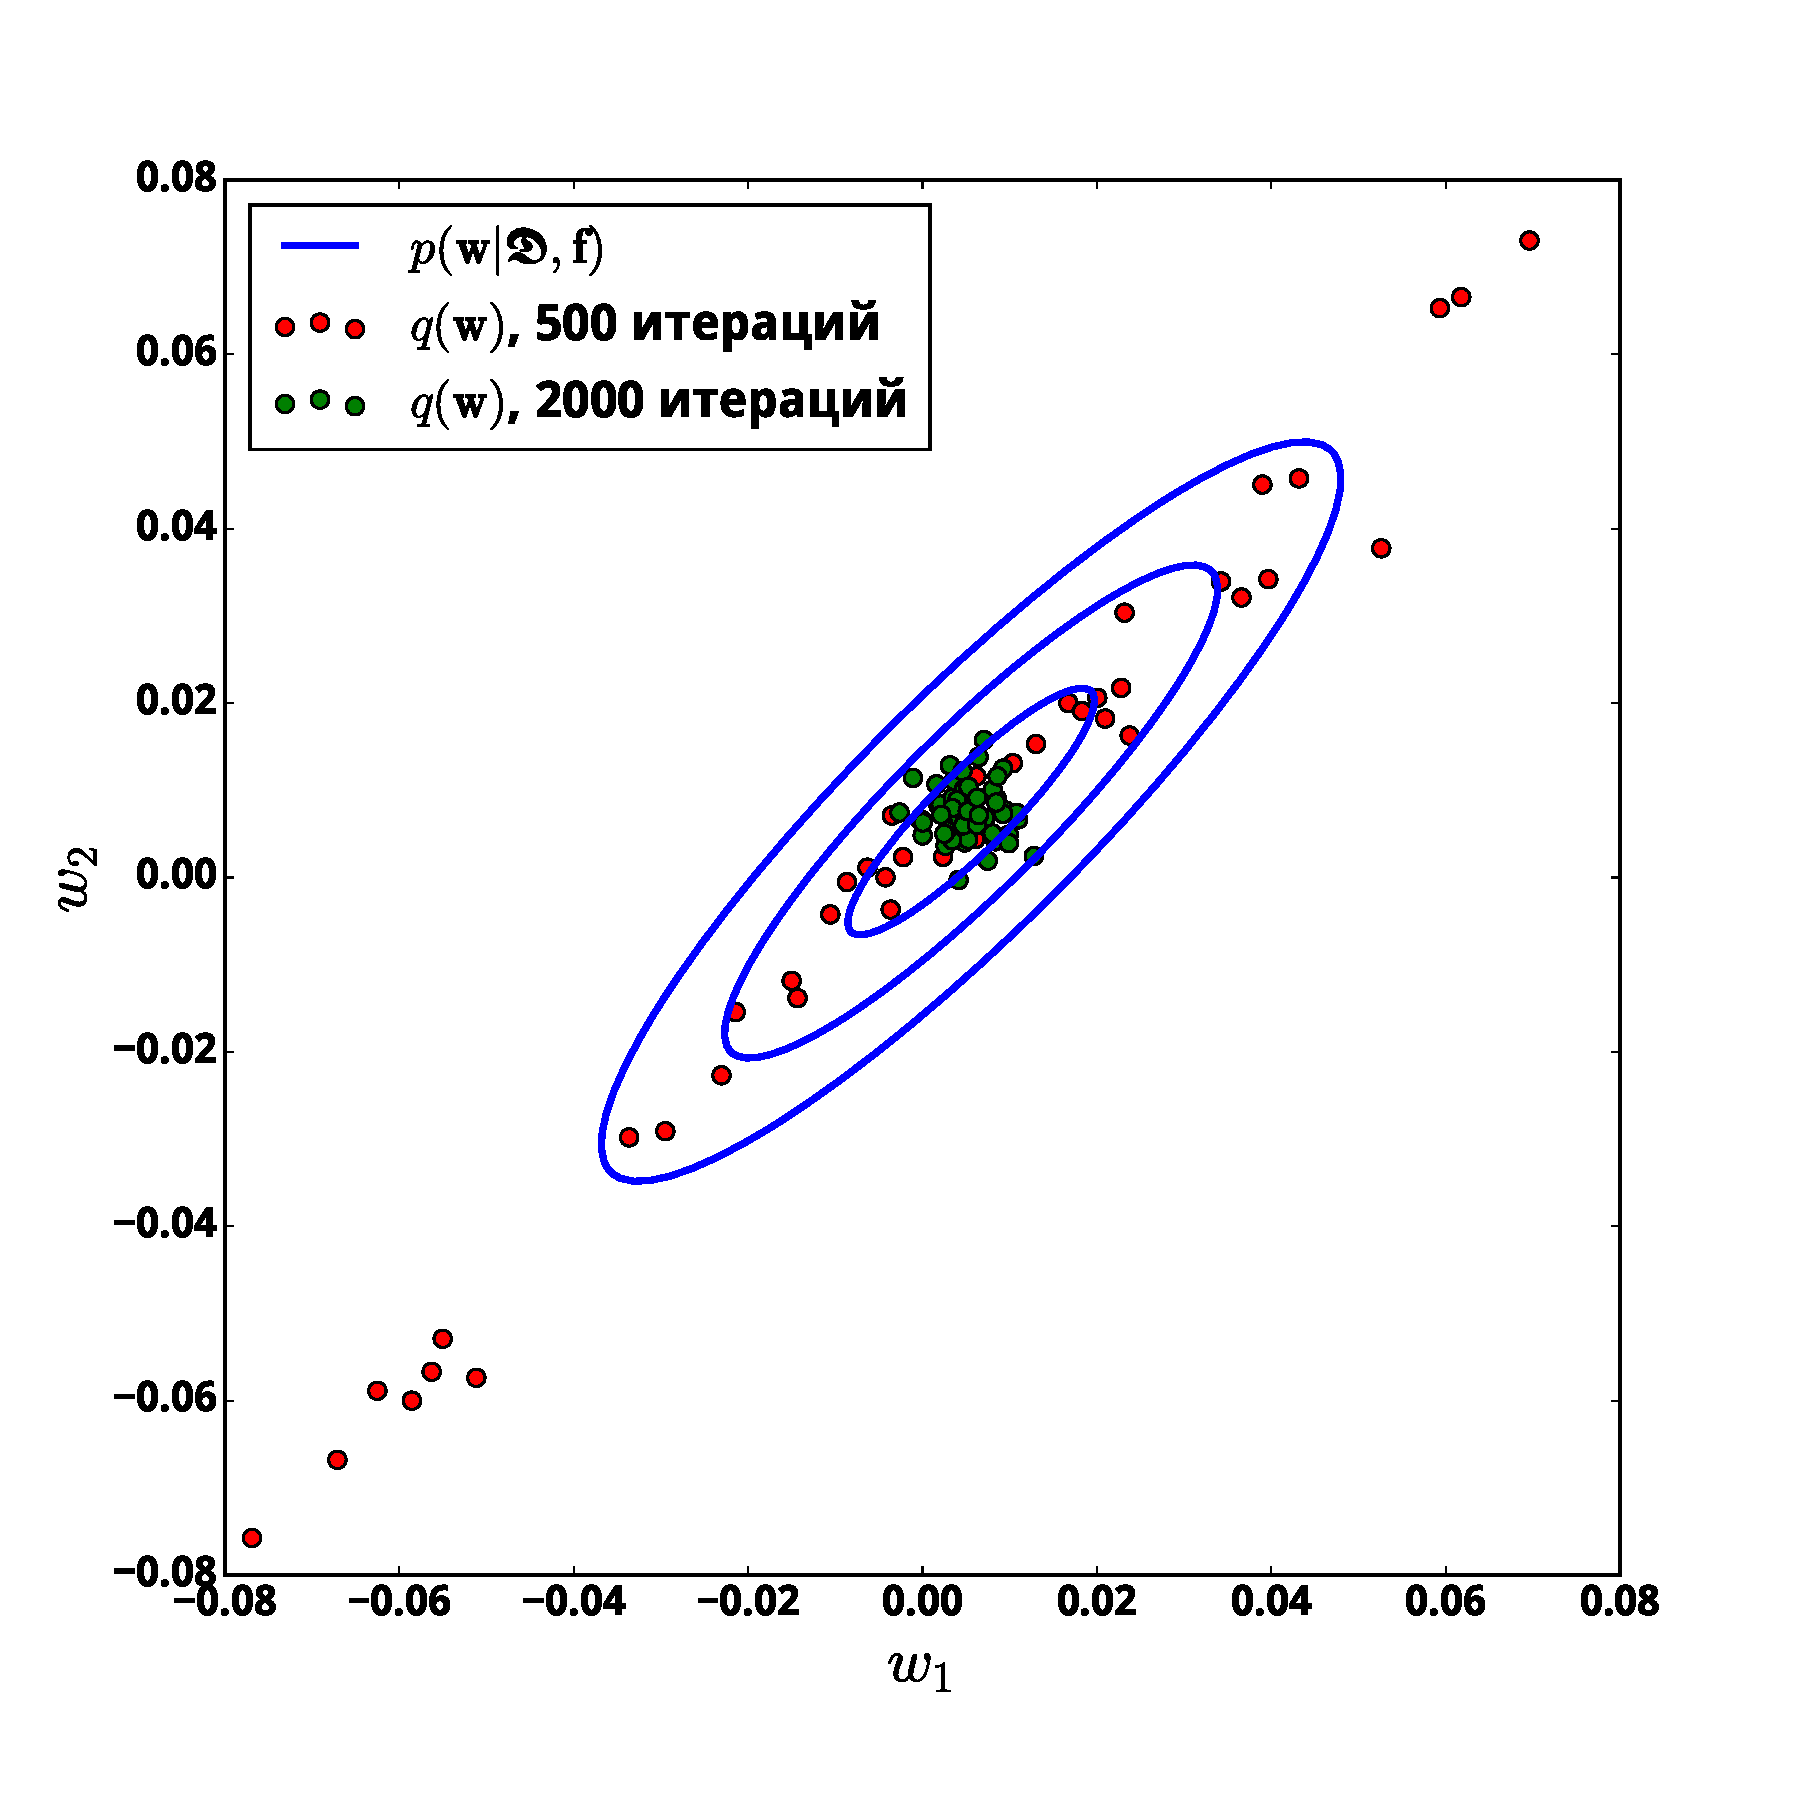
\includegraphics[width=0.35\textwidth]{sgd_estimate.pdf}} 
 \subfloat[Оценка начала переобучения]{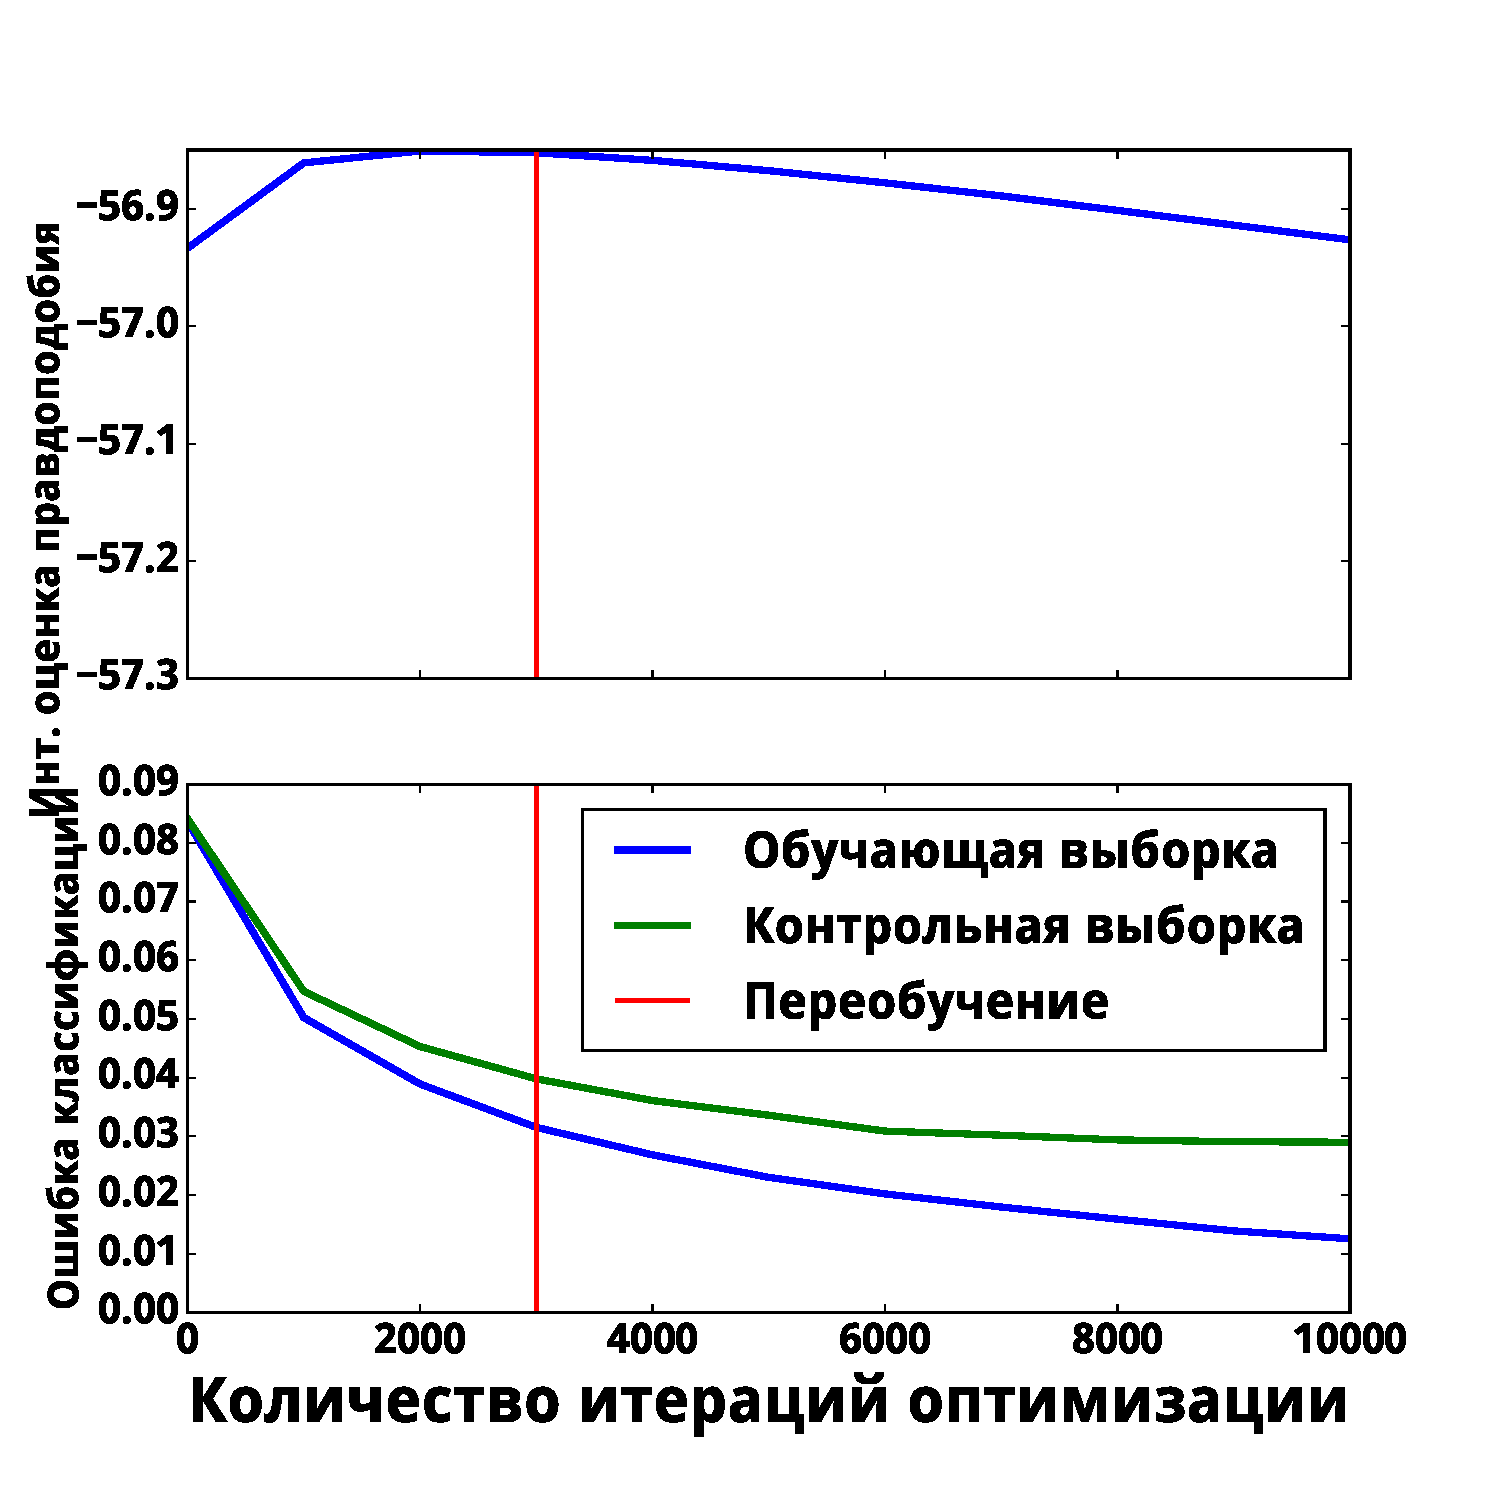
\includegraphics[width=0.35\textwidth]{sgd_show.pdf}}
\label{fig:1}\qquad
\end{figure}
\end{frame}


\begin{frame}{Задача оптимизации гиперпараметров}
Задана дифференцируемая по параметрам модель, приближающая зависимую переменную~$y$:
\[
	\mathbf{f}(\mathbf{w}, \mathbf{x}):\mathbb{W} \times \mathbb{X} \to \mathbb{Y}, \quad \mathbf{w} \in \mathbb{W}
\]

Пусть $\boldsymbol{\theta} \in \mathbb{R}^u$ --- вариационные параметры распределения.\\
$L( \boldsymbol{\theta}| \mathbf{h}, \mathbf{X}, \mathbf{y})$ ---  дифференцируемая функция потерь  по которой производится оптимизация функции ${f}$. \\
$Q(\mathbf{h}| \boldsymbol{\theta}, \mathbf{X}, \mathbf{y} )$ ---  дифференцируемая функция определяющая итоговое качество модели ${f}$.\\

Требуется найти параметры $\boldsymbol{\theta}^{*}$ и гиперпараметры $\mathbf{h}$ модели, доставляющие минимум следующему функционалу:
$$
    \mathbf{h}^{*} = \argmin_{\mathbf{h} \in \mathbb{H}} Q(\mathbf{h}|  \boldsymbol{\theta}^{*}, \mathbf{X}, \mathbf{y} ),
$$
$$
	\boldsymbol{\theta}^{*}(\mathbf{h}) =  \argmin_{\boldsymbol{\theta} \in \mathbb{R}^u} L(\boldsymbol{\theta}|  \mathbf{h},  \mathbf{X}, \mathbf{y}),
$$
\end{frame}


\begin{frame}{Байесовский вывод}
\textit{Первый уровень:}
\[
{\boldsymbol{\theta}}^{*} = \argmax \bigl(-L\bigr) = p(\mathbf{w}|\mathbf{X}, \mathbf{y}, \mathbf{h}) = \frac{p(\mathbf{y}|\mathbf{X},\mathbf{w})p(\mathbf{w}|\mathbf{h})}{p(\mathbf{y}|\mathbf{X},\mathbf{h})}.
\]
\textit{Второй уровень:}
\[
p(\mathbf{h}|\mathbf{X}, \mathbf{y}) \propto p(\mathbf{y}|\mathbf{X},\mathbf{h})p(\mathbf{h}).
\]

Полагая распределение параметров $p(\mathbf{h})$ равномерным на некоторой большой окрестности, получим задачу оптимизации гиперпараметров:
\begin{equation}
\label{eq:bayes2}
	p(\mathbf{y}|\mathbf{X},\mathbf{h}) = \int_{\mathbf{w} \in \mathbb{R}^u} p(\mathbf{y}|\mathbf{X}, \mathbf{w}) p(\mathbf{w}|\mathbf{h}) = -Q \to \max_{[\alpha_1, \dots, \alpha_n] \in \mathbb{R}^{n}}.
\end{equation}
\end{frame}

\begin{frame}{Другие примеры $L,Q$}

\begin{itemize}
\item Кросс-валидация ($L$ --- ошибка на обучении, $Q$ --- на контроле);
\item вариационная оценка ($L=Q=\text{ELBO}$).
\end{itemize}
\end{frame}


\begin{frame}{Формальная постановка задачи: градиентная оптимизация}
\begin{block}{Определение}
Пусть задан оператор $T$, проводящий $\eta$ шагов оптимизации по функции $L$:
\begin{equation}
\label{eq:gd}
	{\boldsymbol{\theta}}^{*} = T \circ T \circ \dots \circ T(\boldsymbol{\theta}^0, \mathbf{h}) = T^\eta(L, \boldsymbol{\theta}_0, \mathbf{h}),
\end{equation}
где 
$\beta$ --- длина шага градиентного спуска, $\boldsymbol{\theta}^0$ --- начальное значение параметров $\boldsymbol{\theta}$.
\end{block}


Перепишем итоговую задачу оптимизации:
\[
	\mathbf{h}^{*} = \argmin_{\mathbf{h} \in \mathbb{R}^h} Q( T^\eta(L, \boldsymbol{\theta}_0, \mathbf{h})).
\]



\end{frame}


\begin{frame}{RMAD, Maclaurin et. al, 2015 }
\begin{columns}
\begin{column}{0.5\textwidth}
\begin{enumerate}
\item Провести $\eta$ шагов оптимизации: $\boldsymbol{\theta} = T(\boldsymbol{\theta}_0, \mathbf{A}^{-1})$.
\item Положим $\hat{\nabla} \mathbf{A}^{-1} = \nabla_\mathbf{A}^{-1} Q(\boldsymbol{\theta}, \mathbf{A}^{-1}).$ 
\item Положим $d\mathbf{v} = \mathbf{0}.$
\item Для $\tau = \eta \dots 1 $ повторить:
\item $\boldsymbol{\theta}^{\tau-1} =  \boldsymbol{\theta}^{\tau} - \gamma\mathbf{v}^{\tau}.$
\item $\mathbf{v}^{\tau-1} =\mathbf{v}^{\tau} + \gamma \hat{\nabla}_{\boldsymbol{\theta}}.$
\item $d\mathbf{v} =  \gamma \hat{\nabla}_{\boldsymbol{\theta}}$.
\item $\hat{\nabla} \mathbf{A}^{-1} =  \hat{\nabla} \mathbf{A}^{-1} - d\mathbf{v}\nabla_{\mathbf{A}^{-1}} \nabla_{\boldsymbol{\theta}} Q$.
\item $\hat{\nabla} \boldsymbol{\theta}  = \hat{\nabla} \boldsymbol{\theta}  - d\mathbf{v}\nabla_{\boldsymbol{\theta}} \nabla_{\boldsymbol{\theta}} Q$.
\end{enumerate}
\end{column}

\begin{column}{0.5\textwidth}
Алгоритм RMAD основывается на Reverse-mode differentiation.
\begin{figure}
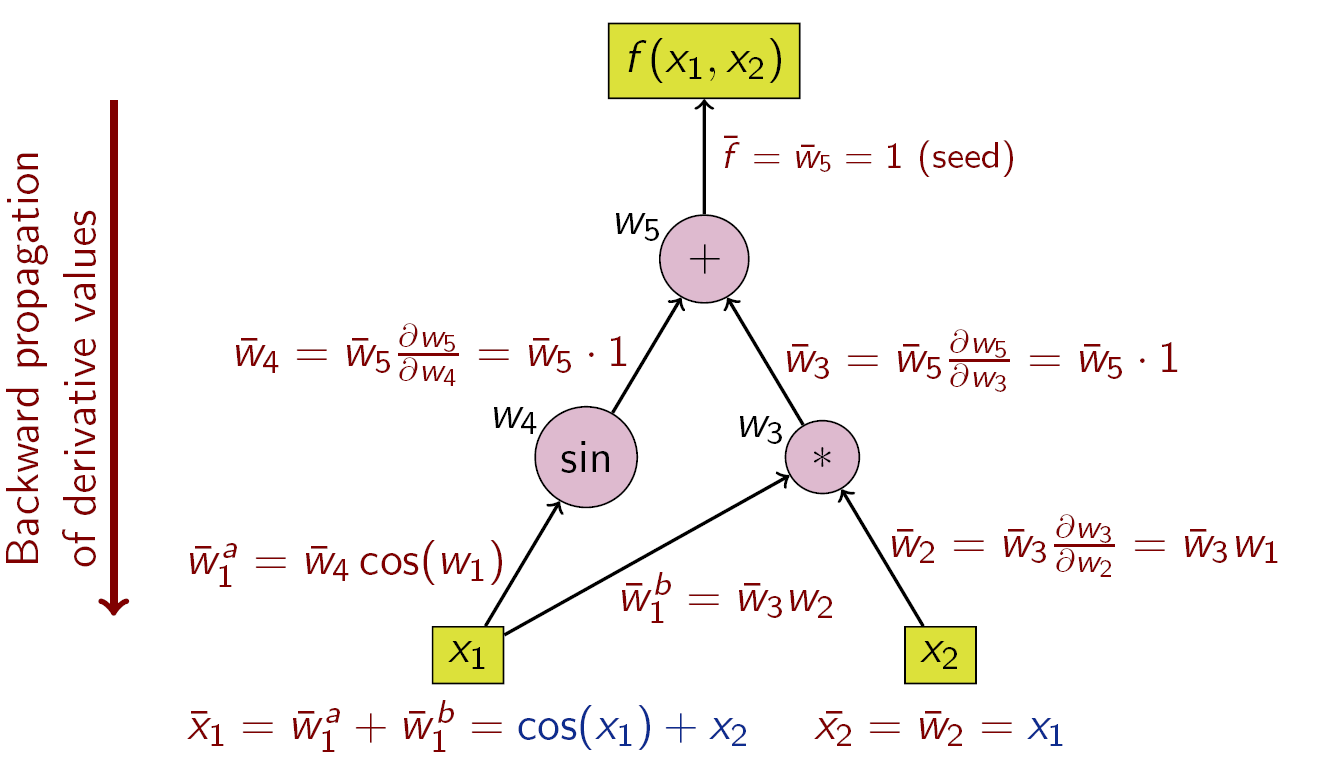
\includegraphics[width=\textwidth]{rmd.png}
\end{figure}
\end{column}
\end{columns}
\end{frame}


\begin{frame}{Эксперименты: полиномы}
\begin{figure}
  \centering
  \subfloat[Кросс-валидация]{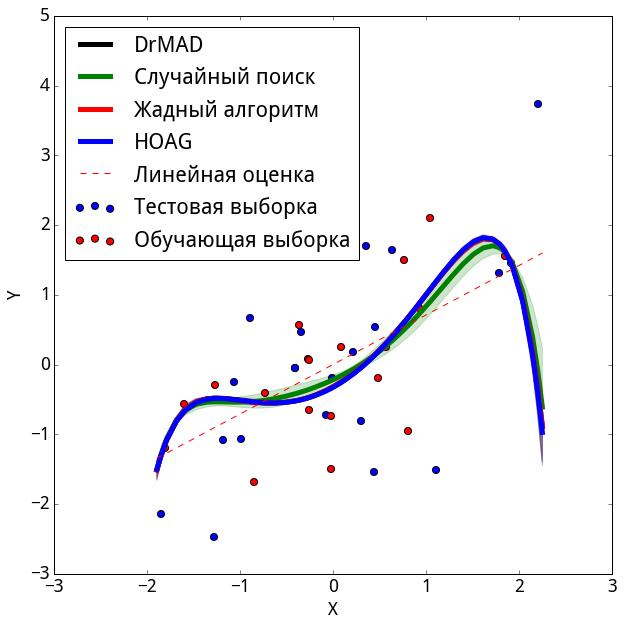
\includegraphics[width=0.42\textwidth]{poly_cv.png}} 
 \subfloat[Evidence]{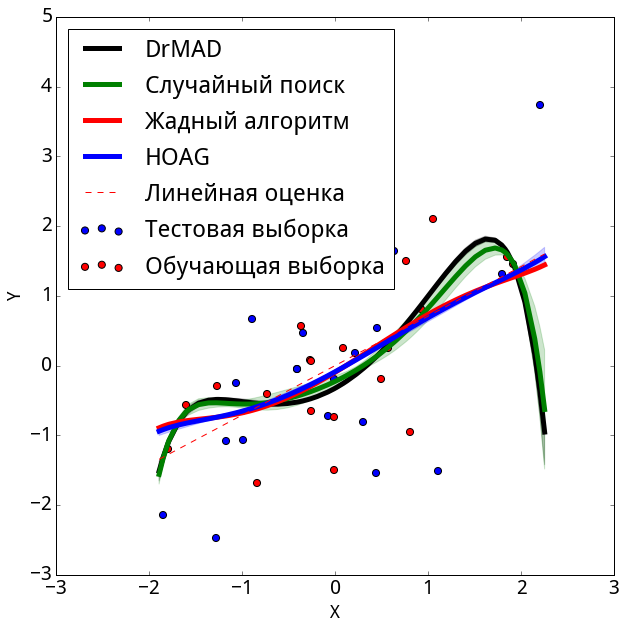
\includegraphics[width=0.42\textwidth]{poly_var.png}}
\label{fig:1}\qquad

\end{figure}
\end{frame}


\begin{frame}{Задача выбора структуры модели}
\small
Однослойная нейросеть:
\[
    \mathbf{f}(\mathbf{x}) = \text{softmax}\left(\mathbf{W}_0^\text{T}\mathbf{f}_1(\mathbf{x})\right), \quad f(\mathbf{x}): \mathbb{R}^n \to [0,1]^{|\mathbb{Y}|}, \quad \mathbf{x} \in \mathbb{R}^n.
\]
\[
\]
\[
\mathbf{f}_1(\mathbf{x}) = {\gamma}_{0,1}^{1}\mathbf{g}_{0,1}^{1}(\mathbf{x})+\dots+{\gamma}_{0,1}^{K}\mathbf{g}_{0,1}^{K}(\mathbf{x})= {\gamma}_{0,1}^{1}\boldsymbol{\sigma}(\mathbf{W}_1^\text{T}\mathbf{x}) + \dots +  {\gamma}_{0,1}^{K}\boldsymbol{\sigma}(\mathbf{W}_K^\text{T}\mathbf{x}),
\]
где $\mathbf{W} = [\mathbf{W}_0,\mathbf{W}_1, \dots, \mathbf{W}_K]^\text{T}$ --- матрицы параметров, $\{\mathbf{g}^{i}_{0,1}\}_{i=1}^K$ --- базовые функции скрытого слоя нейросети.~\\~\\

\textbf{Структурные параметры:}  $\boldsymbol{\Gamma} = [\boldsymbol{\gamma}_{0,1}]$.\\
\textbf{Структура модели} задается вершиной $K$-мерного симплекса.
    
\end{frame}

\begin{frame}{Задача выбора структуры модели: два скрытых слоя}
\small
Двухслойная нейросеть:
\[
    \mathbf{f}(\mathbf{x}) = \text{softmax}\left(\mathbf{W}^\text{T}\textcolor{red}{\mathbf{f}_2}(\mathbf{x})\right), \quad f(\mathbf{x}): \mathbb{R}^n \to [0,1]^{|\mathbb{Y}|}, \quad \mathbf{x} \in \mathbb{R}^n.
\]
\[
\textcolor{red}{
\mathbf{f}_2(\mathbf{x}) = {\gamma}_{1,2}^{1}\mathbf{g}_{1,2}^{1}(\mathbf{f}_1(\mathbf{x}))+\dots+{\gamma}_{1,2}^{K}\mathbf{g}_{1,2}^{K}(\mathbf{f}_1(\mathbf{x}))= {\gamma}_{1,2}^{1}\boldsymbol{\sigma}(\mathbf{W}_{K+1}^\text{T}\mathbf{f}_1(\mathbf{x})) + \dots +  {\gamma}_{1,2}^{K}\boldsymbol{\sigma}(\mathbf{W}_{2K}^\text{T}\mathbf{f}_1(\mathbf{x})),}
\]
\[
\mathbf{f}_1(\mathbf{x}) = {\gamma}_{0,1}^{1}\mathbf{g}_{0,1}^{1}(\mathbf{x})+\dots+{\gamma}_{0,1}^{K}\mathbf{g}_{0,1}^{K}(\mathbf{x})= {\gamma}_{0,1}^{1}\boldsymbol{\sigma}(\mathbf{W}_1^\text{T}\mathbf{x}) + \dots +  {\gamma}_{0,1}^{K}\boldsymbol{\sigma}(\mathbf{W}_K^\text{T}\mathbf{x}),
\]

где $\mathbf{W} = [\mathbf{W}_0,\textcolor{red}{\mathbf{W}_1, \dots, \mathbf{W}_{2K}}]^{\text{T}}$ --- матрицы параметров, $\{\mathbf{g}^{i}_{0,1}, \textcolor{red}{\mathbf{g}^{i}_{1,2}\}_{i=1}^K}$ --- базовые функции скрытых слоев нейросети.~\\~\\

\textbf{Структурные параметры:} $\boldsymbol{\Gamma} = [\boldsymbol{\gamma}_{0,1}, \textcolor{red}{\boldsymbol{\gamma}_{1,2}}]$.\\
\textbf{Структура модели} задается вершинами \textcolor{red}{двух} $K$-мерных симплексов.
\end{frame}


        


\begin{frame}{Графовое представление модели глубокого обучения}
\begin{block}{Определение}
Задан  граф $(V,E)$. Для каждого ребра $(j,k) \in E$ определен вектор базовых функций  мощности $K^{j,k}$: $$\mathbf{g}^{j,k} = [\mathbf{g}^{j,k}_0, \dots, \mathbf{g}^{j,k}_{K^{j,k}}]$$. Пусть для каждой вершины $v \in V$ определена функция агрегации $\textbf{agg}_v$.\\ Граф $(V, E)$ в совокупности со множестом векторов базовых функций $\{\mathbf{g}^{j,k}, (j,k) \in E\}$ и множеством функций агрегаций $\{ \textbf{agg}_v, {v \in V}\}$ называется \textit{параметрическим семейством моделей} $\mathfrak{F}$, если функция, задаваемая как 
\begin{equation}
\label{eq:modelfam}
    \mathbf{f}_k(\mathbf{x}) = \textbf{agg}_k\left(\{ \langle \boldsymbol{\gamma}^{j,k}, \mathbf{g}^{j,k} \rangle \left(\mathbf{f}_j(\mathbf{x})\right)| j \in \text{Adj}(v_k)\}\right), \quad \mathbf{f}_0(\mathbf{x}) = \mathbf{x}
\end{equation}
является моделью при любых значениях векторов, $\boldsymbol{\gamma}^{j,k} \in [0,1]^{K^{j,k}}$.

\end{block}
\end{frame}

\begin{frame}{Пример: двуслойная нейросеть}
\begin{figure}
\small
\begin{tikzpicture}[node distance=cm, auto]
  %\tikzstyle{every state}=[fill=red,draw=none,text=white]

  \node (f0)  at (1,6)                  {$\mathbf{f}_0(\mathbf{x}) = \mathbf{x}$};
  %\node (g11) at (6,3)                    {$\mathbf{g}^{1,1}(\mathbf{x})$};% = \text{Conv}(\mathbf{x}, 3, 32, 1)$};
  %\node (g12)  at (6,9)                   {$\mathbf{g}^{1,2}(\mathbf{x})$};% = \text{Conv}(\mathbf{x}, 4, 32, 1)$};
  \node (f1)  at (5,6)                 {$\mathbf{f}_1(\mathbf{x})$};% = \gamma^{1,1}\mathbf{g}^{1,1}(\mathbf{x}) +  \gamma^{1,2}\mathbf{g}^{1,2}(\mathbf{x})$};
  %\node (g21) at (12,6)                   {$\mathbf{g}^{2,1}(\mathbf{x})$};% = \boldsymbol{\sigma}(\mathbf{w}^{2,1}\mathbf{x})$};
  \node (f2)  at (10,6)                   {$\mathbf{f}_2(\mathbf{x})$};% = \gamma^{2,1}\mathbf{g}^{2,1}(\mathbf{x})$};
  \path[->]  (f0) edge [bend left=50] node {$\mathbf{g}^{0,1}_0(\mathbf{x}) = \boldsymbol{\sigma}(\mathbf{w}^{0,1}_0\mathbf{x})$}(f1);
  \path[->] (f0)  edge[bend right=50] node[below] {$\mathbf{g}^{0,1}_1(\mathbf{x}) = \boldsymbol{\sigma}(\mathbf{w}^{0,1}_1\mathbf{x})$}(f1);
  \path[->] (f1)  edge node {$\mathbf{g}^{1,2}_0(\mathbf{x}) = \textbf{softmax}(\mathbf{w}^{1,2}_0\mathbf{x})$}(f2);       
  \draw[->] (f1) to (f2);
 
\end{tikzpicture}

\end{figure}
\end{frame}

\begin{frame}{Пример: сверточная сеть}
\small
\begin{figure}
\begin{tikzpicture}[node distance=0.5cm, auto]
  %\tikzstyle{every state}=[fill=red,draw=none,text=white]

  \node (f0)  at (1,6)                  {$\mathbf{f}_0(\mathbf{x}) = \mathbf{x}$};
  %\node (g11) at (6,3)                    {$\mathbf{g}^{1,1}(\mathbf{x})$};% = \text{Conv}(\mathbf{x}, 3, 32, 1)$};
  %\node (g12)  at (6,9)                   {$\mathbf{g}^{1,2}(\mathbf{x})$};% = \text{Conv}(\mathbf{x}, 4, 32, 1)$};
  \node (f1)  at (5,6)                 {$\mathbf{f}_1(\mathbf{x})$};% = \gamma^{1,1}\mathbf{g}^{1,1}(\mathbf{x}) +  \gamma^{1,2}\mathbf{g}^{1,2}(\mathbf{x})$};
  %\node (g21) at (12,6)                   {$\mathbf{g}^{2,1}(\mathbf{x})$};% = \boldsymbol{\sigma}(\mathbf{w}^{2,1}\mathbf{x})$};
  \node (f2)  at (10,6)                   {$\mathbf{f}_2(\mathbf{x})$};% = \gamma^{2,1}\mathbf{g}^{2,1}(\mathbf{x})$};
  \path[->]  (f0) edge [bend left=50] node {$\mathbf{g}^{0,1}_0(\mathbf{x}) = \textbf{Conv}(\mathbf{x}, c_0, c_1)$}(f1);
  \path[->] (f0)  edge[bend right=50] node[below] {$\mathbf{g}^{0,1}_1(\mathbf{x}) = \textbf{Conv}(\mathbf{x}, 1, c_1) \circ \textbf{Conv}(\mathbf{x}, c_0, c_2)$}(f1);
  \path[->] (f1)  edge node {$\mathbf{g}^{1,2}_0(\mathbf{x}) = \textbf{softmax}(\mathbf{w}^{2,1}\mathbf{x})$}(f2);            
  \draw[->] (f1) to (f2);
 
\end{tikzpicture}

\end{figure}
\end{frame}



\begin{frame}{Ограничения на структурные параметры}
\begin{figure}
  \centering
{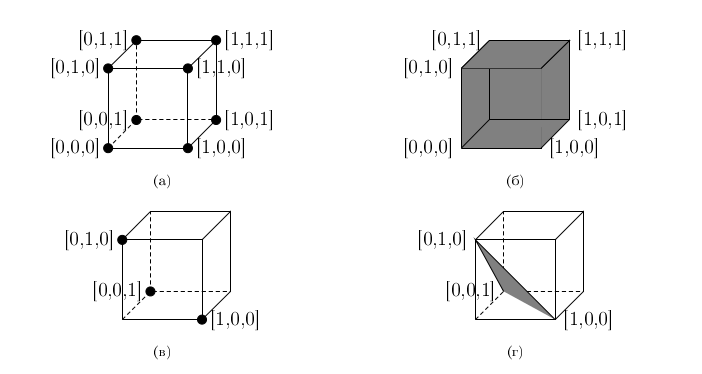
\includegraphics[width=0.8\textwidth]{cubes.png}} 
\end{figure}

\end{frame}





\begin{frame}{Статистические критерии качества модели}


\textbf{Параметрическая сложность} --- наименьшая дивергенция между априорным распределением параметров и апостериорным распределением параметров:
\[
    C_\text{param} = \min_{\mathbf{h}} \text{D}_\text{KL}(p(\mathbf{W}, \boldsymbol{\Gamma}|\mathbf{y}, \mathbf{X})||p(\mathbf{W}, \boldsymbol{\Gamma}||\mathbf{h})).
\]



\textbf{Структурная сложность модели} --- энтропия апостериорного распределения структуры модели:
\[
    C_\text{struct} = -\mathsf{E}_{p} \text{log}~p(\boldsymbol{\Gamma}|\mathbf{y}, \mathbf{X}).
\]

\end{frame}

\iffalse  
\begin{frame}{Выбор оптимальной модели}
\textbf{Основные проблемы выбора оптимальной модели}\\
\begin{itemize}
\item Интеграл правдоподобия $p(\mathbf{y}|\mathbf{X}, \mathbf{h})$ невычислим аналитически.
\item Задача его оптимизации многоэкстремальна и невыпукла.
\end{itemize}
~\\
\textbf{Требуется}\\ 
Предложить метод поиска субоптимального решения задачи оптимизации, обобщающего различные алгоритмы оптимизации:
\begin{itemize}
\item Оптимизация правдоподобия.
\item Последовательное увеличение и снижение сложности модели.
\item Полный перебор вариантов структуры модели.
\end{itemize}

\end{frame} 
   


\begin{frame}{ Распределение на структуре}
Пусть для каждого ребра $(j,k)$ задан нормированный положительный вектор $\boldsymbol{\gamma}_{j,k} \in \mathbb{R}_{+}^{|K_{j,k}|}$, определяющий веса базовых функций из  $\mathbf{g}(j,k)$. Перечислим основные свойства, которыми должно обладать распределение такого вектора:
\begin{enumerate}
\item $p(\boldsymbol{\gamma}^{j,k})$ является непрерывным на симплексе $\Delta^{K^{j,k}-1}$.
\item При устремлении температуры к бесконечности распределение сходится к равномерному: $\lim_{c_{\text{temp}} \to \infty} = p(\boldsymbol{\gamma}^{j,k})| \text{c}_{\text{temp}}) = \mathcal{U}(\Delta^{K^{j,k}-1}).$
\item При устремлении температуры к нулю распределение сходится к сингулярному распределению следующего вида:
$$\lim_{c_{\text{temp}} \to 0}  p(\gamma^{j,k}_k) = m^{j,k}_k,$$ где $\mathbf{m}^{j,k}$ --- параметр распределения.
\end{enumerate}


\end{frame}


\begin{frame}{Варианты распределений}
\begin{enumerate}
\item Дирихле;
\item Гумбель-Софтмакс: 
\[
    \hat{\boldsymbol{\gamma}}_h = \text{exp}\left(\text{log}\left(m_h + \text{Gum}_h\right)c_{\text{temp}}^{-1}\right) \sum_{l=1}^{K_{j,k}} \text{exp}\left(\text{log}\left(m_l + \text{Gum}_l\right)c_{\text{temp}}^{-1}\right),
\]
где $\text{Gum} \sim -\text{log}(-\text{log}~\mathcal{U}(0,1)).$ 
\end{enumerate}

\begin{figure}
  \centering
{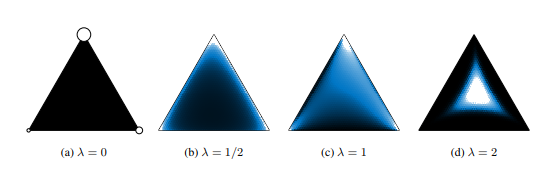
\includegraphics[width=0.8\textwidth]{gs.png}} 
\end{figure}

Maddison et al., 2017.
\end{frame}



\begin{frame}{Оптимизация параметров вариационного распределения}
\footnotesize
Параметры вариационного распределения $q(\mathbf{W}, \boldsymbol{\Gamma}) = q_{\mathbf{W}}(\mathbf{W})q_{\boldsymbol{\Gamma}}(\boldsymbol{\Gamma})$ оптимизируем:
\[
L =
\textcolor{blue}{\mathsf{E}_q \text{log}~{p(\mathbf{y} | \mathbf{X}, \mathbf{W}, \boldsymbol{\Gamma}. \mathbf{A}^{-1}, c_{\text{temp}})}} - \textcolor{red}{c_\text{reg}\text{D}_{KL}\left(p(\mathbf{w}, \boldsymbol{\Gamma} |\mathbf{A}^{-1}, \mathbf{m}, c_{\text{temp}}) || q(\mathbf{W}), q(\boldsymbol{\Gamma})\right)} \to \max_{\mathbf{A}_q, \boldsymbol{\mu}_q, \mathbf{m}_q}.
\]

\begin{block}{Теорема.}
Пусть $c_\text{reg} > 0$ .
Тогда $\frac{1}{m}L(c_\text{reg})$ сходится п.н. к той же функции, что и $\frac{c_\text{reg}}{m_0}L(c_\text{reg}=1)$.
\end{block}
\textbf{Интерпретация: } для достаточно большого $m$ и $c_\text{reg} \neq 1$ оптимизация параметров и гиперпараметров эквивалентна оптимизации ELBO для выборки другой мощности.


\begin{block}{Теорема  [Бахтеев, 2018].}
Пусть $\boldsymbol{\Gamma}_1$ и $\boldsymbol{\Gamma}_2$ --- реализации $\boldsymbol{\Gamma}$, такие что:
\begin{itemize}
\item $\boldsymbol{\Gamma}_1 \in \bar{\Delta}(\boldsymbol{\Gamma})$.
\item $\boldsymbol{\Gamma}_2 \not \in \bar{\Delta}(\boldsymbol{\Gamma})$.
\end{itemize} 
Тогда для любых положительно определенных матриц $\mathbf{A}_1$ и $\mathbf{A}_2$ и векторов $\mathbf{m}_1, \mathbf{m}_2, \text{min}(\mathbf{m}_1)>0$ справедлива следующее отношение апостериорных вероятностей:
$$\lim_{c_\text{temp} \to 0} \frac{p(\boldsymbol{\Gamma}_2, \mathbf{W}_2|\mathbf{y},  \mathbf{X},\mathbf{A}_1,\mathbf{m}_2, {c_\text{temp}})}{p(\boldsymbol{\Gamma}_1,  \mathbf{W}|\mathbf{y}, \mathbf{X},\mathbf{A}_1,\mathbf{m}_1, {c_\text{temp}})} = \infty.$$
\end{block}
\end{frame}


\begin{frame}{Оптимизация параметров априорного распределения}
\small
Гиперпараметры $\mathbf{A}, \mathbf{m}$ оптимизируем:
\[
Q = \textcolor{blue}{c_\text{train}\mathsf{E}_q \text{log}~{p(\mathbf{y} | \mathbf{X}, \mathbf{W}, \boldsymbol{\Gamma}. \mathbf{A}^{-1}, c_{\text{prior}})}}
 - \textcolor{red}{c_\text{prior}\text{D}_{KL}(p(\mathbf{W}, \boldsymbol{\Gamma} |\mathbf{A}^{-1}, \mathbf{m}, c_{\text{temp}}) || q(\mathbf{W}, \boldsymbol{\Gamma}))} -\]
\[
 - \textcolor{OliveGreen}{c_{\text{comb}}\sum_{p' \in \mathbf{P}} \text{D}_{KL}(\boldsymbol{\Gamma} | p')} \to \max, 
\]
где $\mathbf{P}$ --- множество (возможно пустое) распределений на структуре модели.
\begin{itemize}
\item $\textcolor{blue}{c_\text{train}}$ --- коэффициент правдоподобия выборки;
\item $\textcolor{red}{c_\text{prior}}$ --- коэффициент регуляризации модели;
\item $\textcolor{OliveGreen}{c_{\text{comb}}}$ --- коэффициент перебора структуры.
\end{itemize}
\end{frame}

\begin{frame}{Общая задача оптимизации}
\small
Общая задача оптимизации --- двухуровневая:
\[
\hat{\mathbf{A}}, \hat{\mathbf{m}} = \argmax_{\mathbf{A}, \mathbf{m}} Q = 
\]
\[
= \textcolor{blue}{c_\text{train}\mathsf{E}_{\hat{q}} \text{log}~{p(\mathbf{y} | \mathbf{X}, \mathbf{W}, \boldsymbol{\Gamma}. \mathbf{A}^{-1}, c_{\text{prior}})}}
 - \textcolor{red}{c_\text{prior}\text{D}_{KL}(p(\mathbf{W}, \boldsymbol{\Gamma} |\mathbf{A}^{-1}, \mathbf{m}, c_{\text{temp}}) || \hat{q}(\mathbf{W}, \boldsymbol{\Gamma}))} -\]
\[
 - \textcolor{OliveGreen}{c_{\text{comb}}\sum_{p' \in \mathbf{P}} \text{D}_{KL}(\boldsymbol{\Gamma} | p')}, 
\]
где 
\[
\hat{q} = \argmax_{q} L = 
\textcolor{blue}{\mathsf{E}_q \text{log}~{p(\mathbf{y} | \mathbf{X}, \mathbf{W}, \boldsymbol{\Gamma}. \mathbf{A}^{-1}, c_{\text{temp}})}} - \textcolor{red}{c_\text{reg}\text{D}_{KL}(p(\mathbf{w}, \boldsymbol{\Gamma} |\mathbf{A}^{-1}, \mathbf{m}, c_{\text{temp}}) || q(\mathbf{W}), q(\boldsymbol{\Gamma}))}
\]

\end{frame}





\begin{frame}{Параметрическая сложность}
\small
Обозначим за $F(c_{\text{reg}}, c_{\text{train}}, c_{\text{prior}}, c_{\text{comb}}, \mathbf{P}, c_{\text{temp}})$ множество экстремумов функции $L$ при решении задачи двухуровневой оптимизации.
\begin{block}{Утверждение.}
Пусть $\mathbf{f} \in F(1, 1, c_{\text{prior}}, 0, \varnothing,  c_{\text{temp}} )$.
При устремлении $ c_{\text{prior}}$ к бесконечности параметрическая сложность модели $\mathbf{f}$ устремляется к нулю.
\[
    \lim_{c_{\text{prior}} \to \infty} C_{\text{param}}(\mathbf{f}) = 0.
\]
\end{block}

\begin{block}{Утверждение.}
Пусть $\mathbf{f}_1 \in F(1, 1, c_{\text{prior}}^1, 0, \varnothing,  c_{\text{temp}} ), \mathbf{h}_2 \in F(1, 1, c_{\text{prior}}^2, 0, \varnothing,  c_{\text{temp}})$, $c_{\text{prior}}^1 < c_{\text{prior}}^2$.\\
Пусть вариационные параметры моделей $\mathbf{f}_1$ и $\mathbf{f}_2$ лежат в области $\mathsf{U}$, в которой соответствующие функции $L$ и $Q$ являются локально-выпуклыми.\\ 
Тогда модель $\mathbf{f}_1$ имеет параметрическую сложность, не меньшую чем у $\mathbf{f}_2$.
\[
    C_\text{param}(\mathbf{f}_1) \geq C_\text{param}(\mathbf{f}_2).
\]
\end{block}


\end{frame}

\begin{frame}{Структурная сложность}
\small

\begin{block}{Теорема  [Бахтеев, 2018].}
Пусть для каждого ребра $(i,j)$ семейства моделей $\mathfrak{F}$ априорное распределение $$p(\boldsymbol{\gamma}_{i,j}) =  \lim_{c_{\text{temp}} \to 0} \mathcal{GS}(c_{\text{temp}}).$$
Пусть $c_{\text{reg}} >0, c_{\text{train}} >0, c_{\text{prior}}>0$.
Пусть $\mathbf{f} \in F(c_{\text{reg}}, c_{\text{train}}, c_{\text{prior}}, 0, \varnothing, c_{\text{temp}})$.
Тогда структурная сложность модели $\mathbf{f}$ равняется нулю.
\[
    C_\text{struct}(\mathbf{f}) = 0.
\]
\end{block}

\begin{block}{Утверждение.}
Пусть $\mathbf{f}_1 \in F(c_{\text{reg}}, c_{\text{train}},  c_{\text{prior}}, 0, \varnothing,  c^1_{\text{temp}}), \mathbf{h}_2   \in \lim_{c^2_{\text{temp}} \to \infty} F(c_{\text{reg}}, c_{\text{train}},  c_{\text{prior}}, 0, \varnothing,  c^2_{\text{temp}})$.
Пусть вариационные параметры моделей $f_1$ и $f_2$ лежат в области $U$, в которой соответствующие функции $L$ и $Q$ являются локально-выпуклыми. 
Тогда разница структурных сложностей моделей ограничена выражением:
\[
    C_\text{struct}(\mathbf{f}_1)  - C_\text{struct}(\mathbf{f}_2) \leq \textcolor{blue}{\mathsf{E}_q^1 \text{log}~{p(\mathbf{y} | \mathbf{X}, \mathbf{W}, \boldsymbol{\Gamma}. \mathbf{A}^{-1}, c^1_{\text{temp}})}} - \textcolor{blue}{\mathsf{E}_q^2 \text{log}~{p(\mathbf{y} | \mathbf{X}, \mathbf{W}, \boldsymbol{\Gamma}, \mathbf{A}^{-1})}}.
\]
\end{block}

% Схема доказательства:
% расписываем неравенства вида: L_1 - DKL(q_1|p1) <L_2 - DKL(q_2|p1)
% Замечаем, что при стремлении к бесконечности гумбель превращается в равномерное
% выражаем все в равномерном
% замечаем, что D_KL = Entropy + const для равномерного
% все
\end{frame}


\begin{frame}{Полный перебор}
\small
Пусть для каждого ребра $(i,j)$ семейства моделей $\mathfrak{F}$ априорное распределение $$p(\boldsymbol{\gamma}_{i,j}) =  lim_{c_{\text{temp}} \to 0} \mathcal{GS}(c_{\text{temp}}).$$

Рассмотрим последовательность $\mathbf{P}$, состоящую из $N = \prod_{(j,k) \in E} K_{j,k}$ моделей, полученных в ходе оптимизаций вида:
$$f_1 \in F(c_{\text{reg}}, 0, 0, \varnothing, c_{\text{comb}},  c_{\text{temp}}),$$
$$f_2 \in F(c_{\text{reg}}, 0, 0, \{q_1(\boldsymbol{\Gamma})\},  c_{\text{comb}},  c_{\text{temp}}),$$
$$f_3 \in F(c_{\text{reg}}, 0, 0, \{q_1(\boldsymbol{\Gamma}), q_2(\boldsymbol{\Gamma})\},  c_{\text{comb}},  c_{\text{temp}}),$$
где $C_{\text{reg}} > 0,  c_{\text{comb}}>0$.


\begin{block}{Теорема}
Вариационные распределения $q_{\boldsymbol{\Gamma}}$ структур  последовательности $\mathbf{P}$ вырождаются в распределения вида $\delta(\hat{\mathbf{m}})$, где $\hat{\mathbf{m}}$ --- точка на декартовом произведении вершин симплексов структуры модели.

Последовательность соответствует полному перебору структуры $\boldsymbol{\Gamma}$.
\end{block}
\end{frame}
\fi
\end{document}

